\def\year{2016}\relax
%File: formatting-instruction.tex
\documentclass[letterpaper]{article}
\usepackage{aaai16}
\usepackage{times}
\usepackage{helvet}
\usepackage{subfig}
\usepackage{amssymb}
\usepackage{enumitem}
\usepackage{amsmath}
\usepackage{pifont}
\usepackage{multirow}
\usepackage{hyperref}
\usepackage[table,xcdraw]{xcolor}
\usepackage[normalem]{ulem}
\useunder{\uline}{\ul}{}
\usepackage{courier}
\usepackage{graphicx}
\usepackage{epsfig}
\newcommand{\xmark}{\ding{55}}%
\newcommand{\starmark}{\ding{72}}%
\frenchspacing
\setlength{\pdfpagewidth}{8.5in}
\setlength{\pdfpageheight}{11in}
\pdfinfo{
/Title (Learning Topical Social Sensor on Twitter)
/Author (Author1, Author2, Author3}
\setcounter{secnumdepth}{0}  
 \begin{document}
% The file aaai.sty is the style file for AAAI Press 
% proceedings, working notes, and technical reports.
%
\title{Learning Topical Social Sensor}
\author{Authors\\
Affiliations
}
\maketitle
\begin{abstract}
Twitter represents a massively distributed social sensor of a rich underlying topic space that drives its content generation.  Yet Twitter content is so diverse, decentralized, and dynamic in nature, that it is hard to automatically aggregate this topical content.  To address this need, we provide a novel way of learning topical social sensors on Twitter that learn from a provided set of topical hashtags and generalize to identify topical tweets with previously unseen tags.  These learning social sensors leverage a variety of user-based, hashtag-based, term-based, and location-based features for distinguishing topical from non-topical tweets; we further analyze these features to understand which features are most useful and why.  We further assess general global topical trends and how our learning sensors are able to follow these trends by drawing from a rich variety of sources on the Twittersphere to enable a first generation of learning social sensors for Twitter. 
\end{abstract}

\section{Introduction}
Twitter hosts lots of information, on average more than $2,200$ new tweets every second. This can get up to $3$ to $4$ times increase during large events such as tsunami. \footnote{\hyperref[]{https://blog.twitter.com/2011/the-engineering-behind-twitter-s-new-search-experience}}
\begin{itemize}
\item Twitter is a vast sensor of content generated by latent phenonema (e.g., flu, political sentiment, elections, environment).
\item Learning topical social sensors (politicians in NY, road conditions in Toronto) -- very broad topics for which its hard to manually specify a useful query.
\item But there is interesting topical content and wouldn't it be cool if we could learn a social sensor for a targeted topic?
\item Key insight is that hashtags are topical and can be used to bootstrap a supervised learning system that as we will show generalizes well beyond the seed hashtags.
\item Conclusion is a new way to build topical real-time feeds that are otherwise difficult to do with existing Twitter tools (???).
\end{itemize}
section{Learning Topical Social Sensors}

Start off with the questions that we want to answer in this section:

- How to evaluate, labeling (problem of no supervised labels for tweets, indirect via hashtags as topical surrogates, leads to question of hashtag curation)?

- Which classification algorithm is best / most robust for learning topical social sensors?

\section{Dataset Statistics}

We crawled Twitter data using Twitter Streaming API for two years spanning 2013 and 2014 years. This type of crawling provides us with a very sparse set of data, roughly $1\%$ of all tweets \footnote{\hyperref[]{http://allthingsd.com/20101110/twitter-firehose-too-intense-take-a-sip-from-the-garden-hose-or-sample-the-spritzer|}}. The total number of tweets collected is $829,026,458$. In the context of Twitter, we consider a list of $5$ features for each tweet. Each tweet has a $From$, the person who tweeted it, and a $Time$ which is the date information of the tweet. It can also contain 
\begin{itemize}
\item $Hashtag(s)$, keywords specified using \# sign
\item $Mention(s)$, another Twitter username being mentioned using @ sign
\item $Term(s)$, uni-grams which we extract from the 140 characters of the tweet. These uni-grams are later cleaned to remove $Term$s with no meaning (total number of $Term$s before cleaning was $20,234,729$)
\end{itemize}
Table \ref{table:featureStatistics} provides more detail statistics about each feature. For each feature, we reported the count of the feature in our dataset, in addition to maximum, average, median counts of each feature across the tweets. Lower part of the table provides these counts across user dimension meaning that for example a hashtag has been used in average by $10.08$ users. Last part of the table shows the statistics for the hashtag usage of our users e.g., users have used $2$ hashtags in average.

%%%%%%%%%%%%%%%%%%%%%%%%%%%%%%%%%%%%%%%%%%%%%%%%%%%%%%%%%%%%%%%%%%%%%%%%%%%
\begin{figure*}[tbph!]
\centering
\begin{tabular}{ccc}
\begin{tabular}{ccc}
\subfloat[Fig:][Human Caused Disaster]{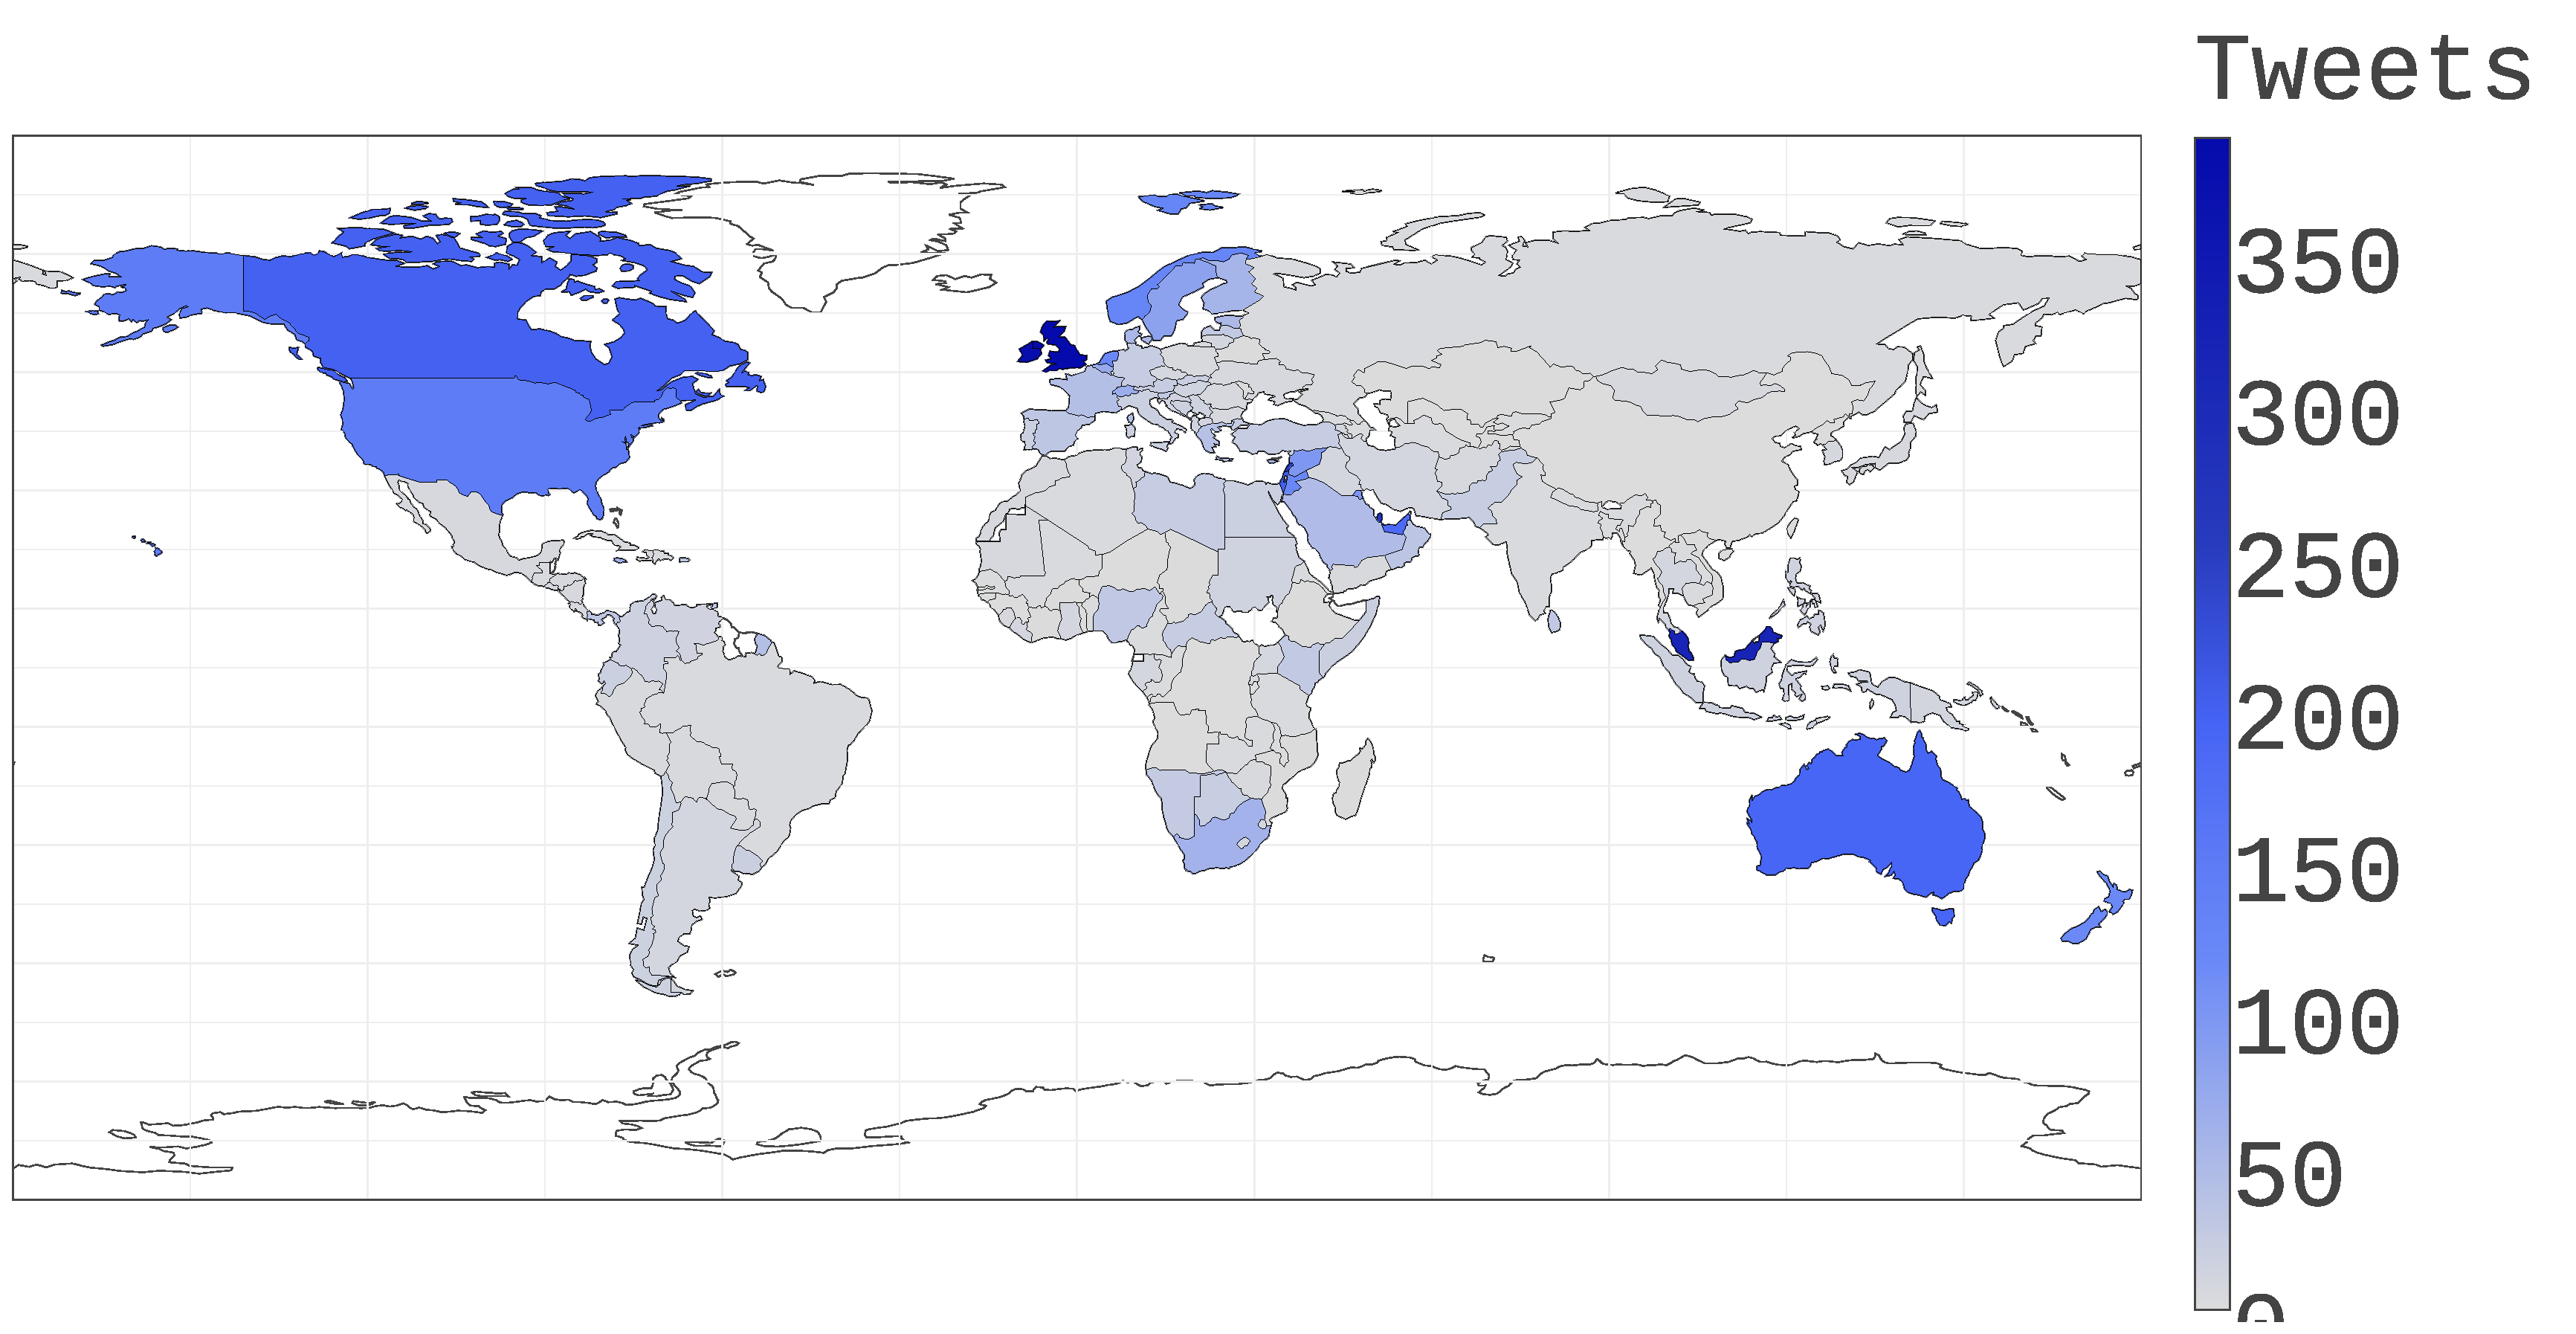
\includegraphics[width=5.3cm]{img/world/socialsensor-world-humancauseddisaster_location.eps}}
\subfloat[Fig:][Iran Deal]{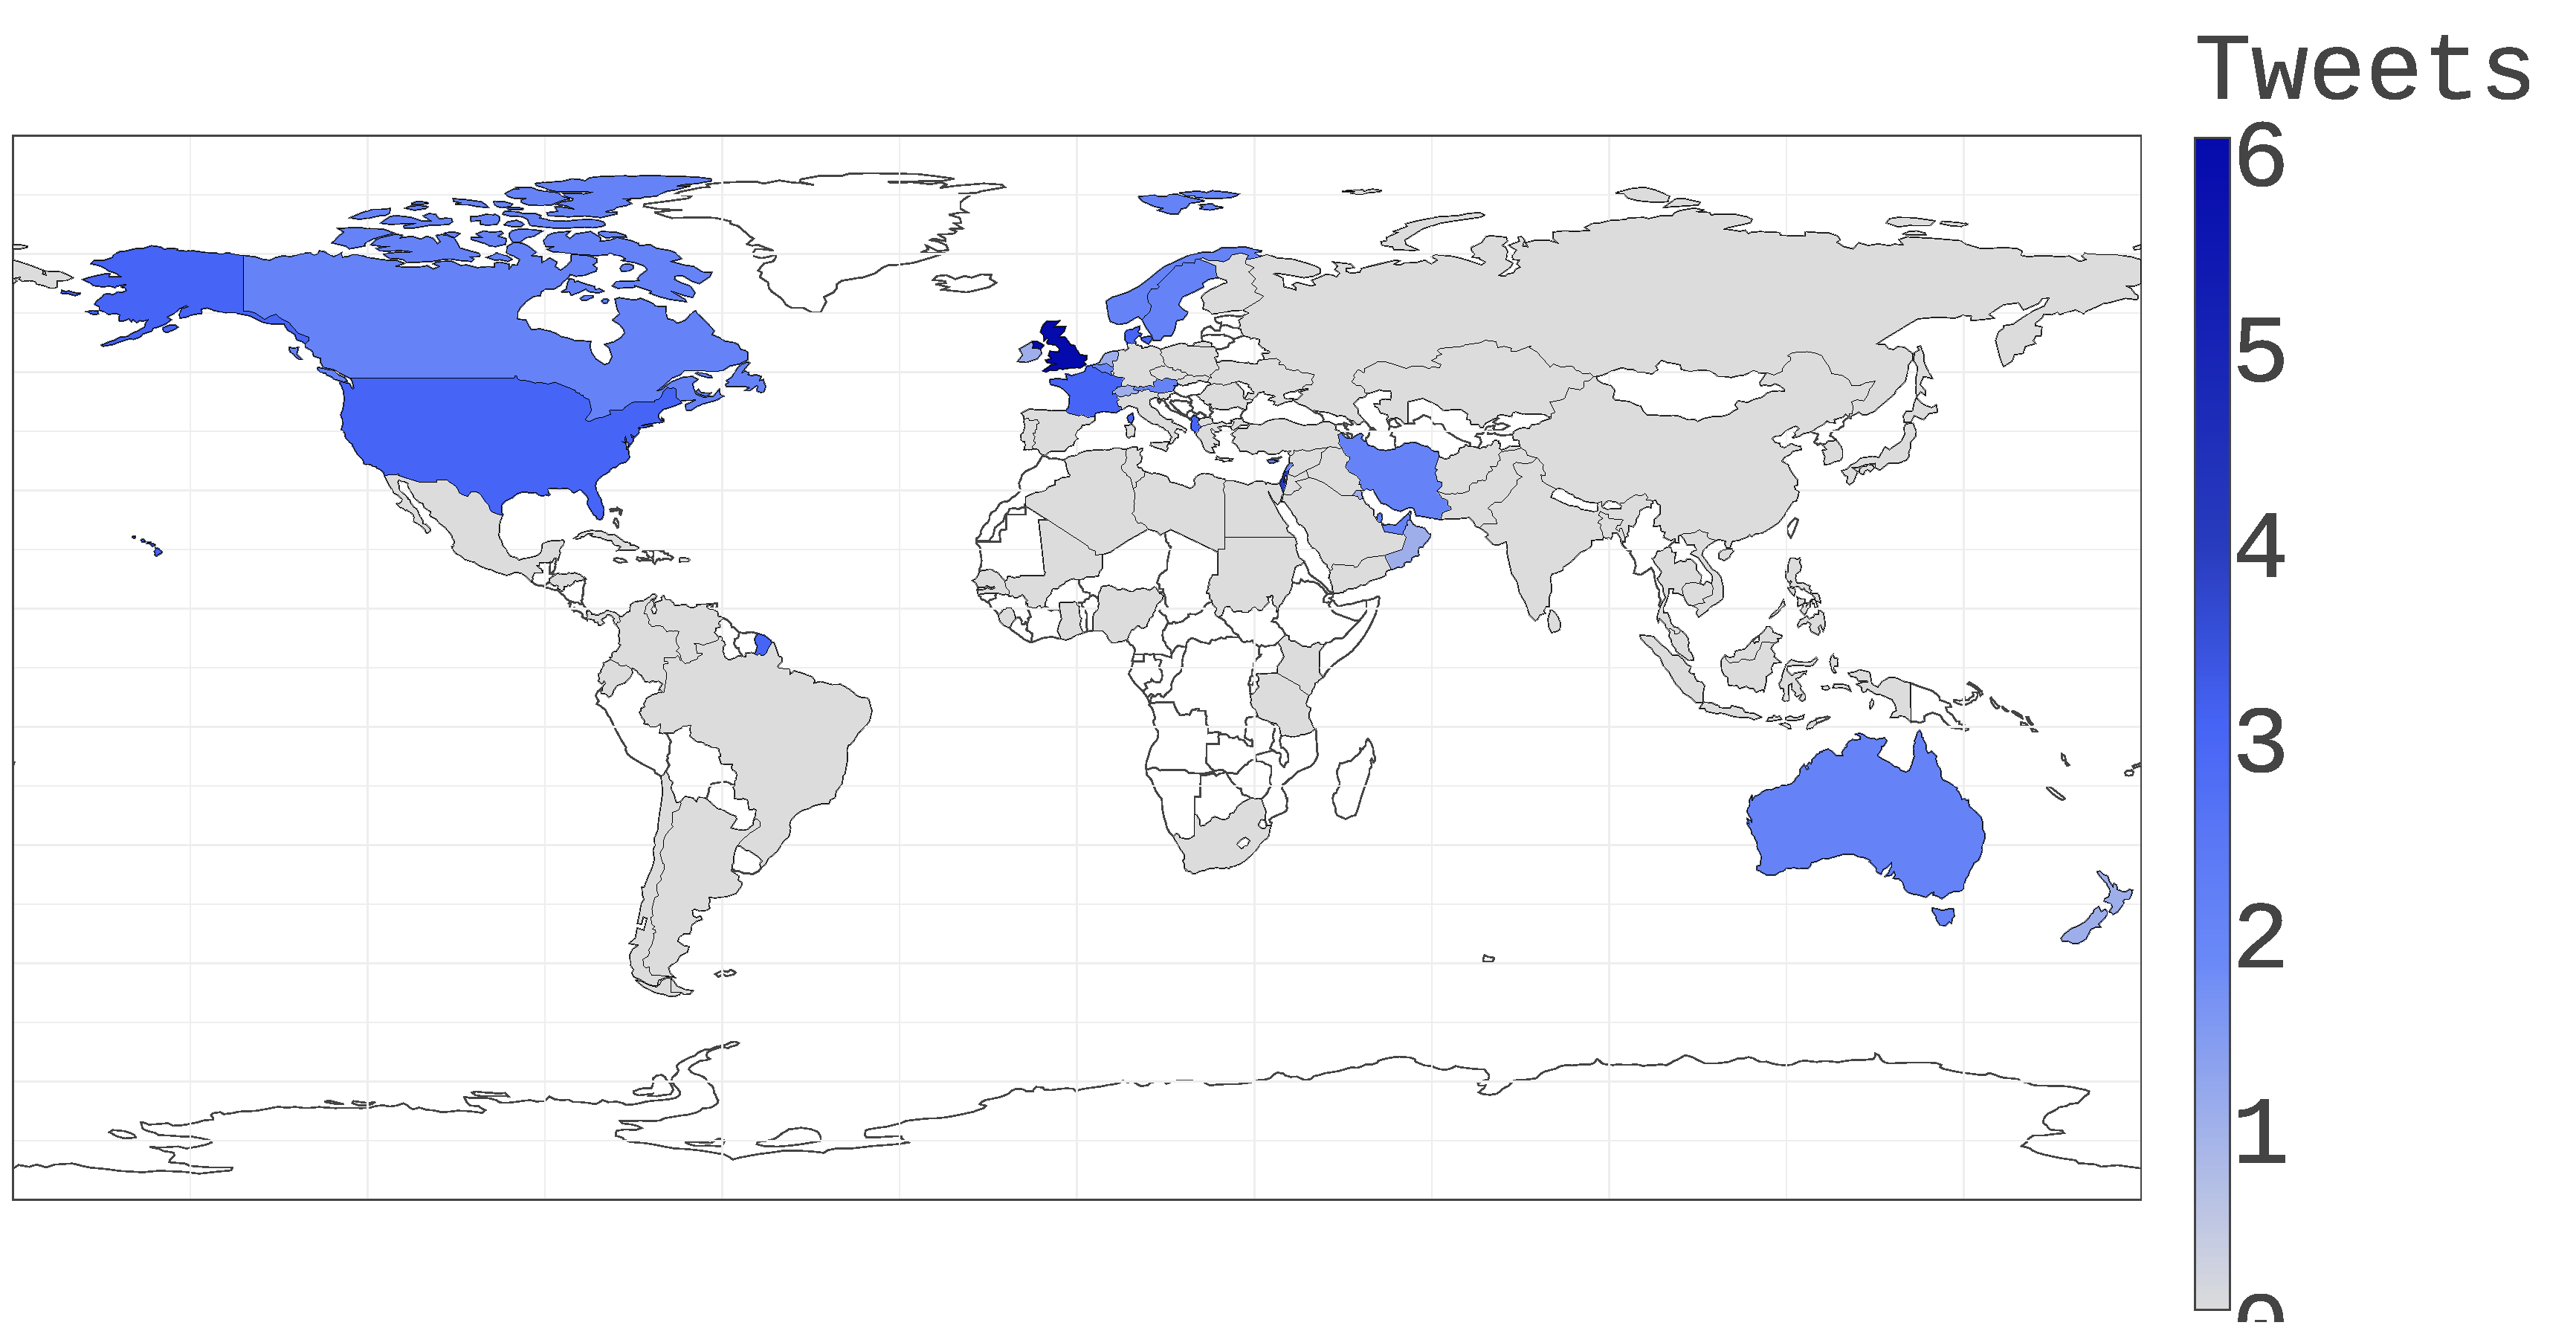
\includegraphics[width=5.3cm]{img/world/socialsensor-world-irannucleardeal_location.eps}}
\subfloat[Fig:][Soccer]{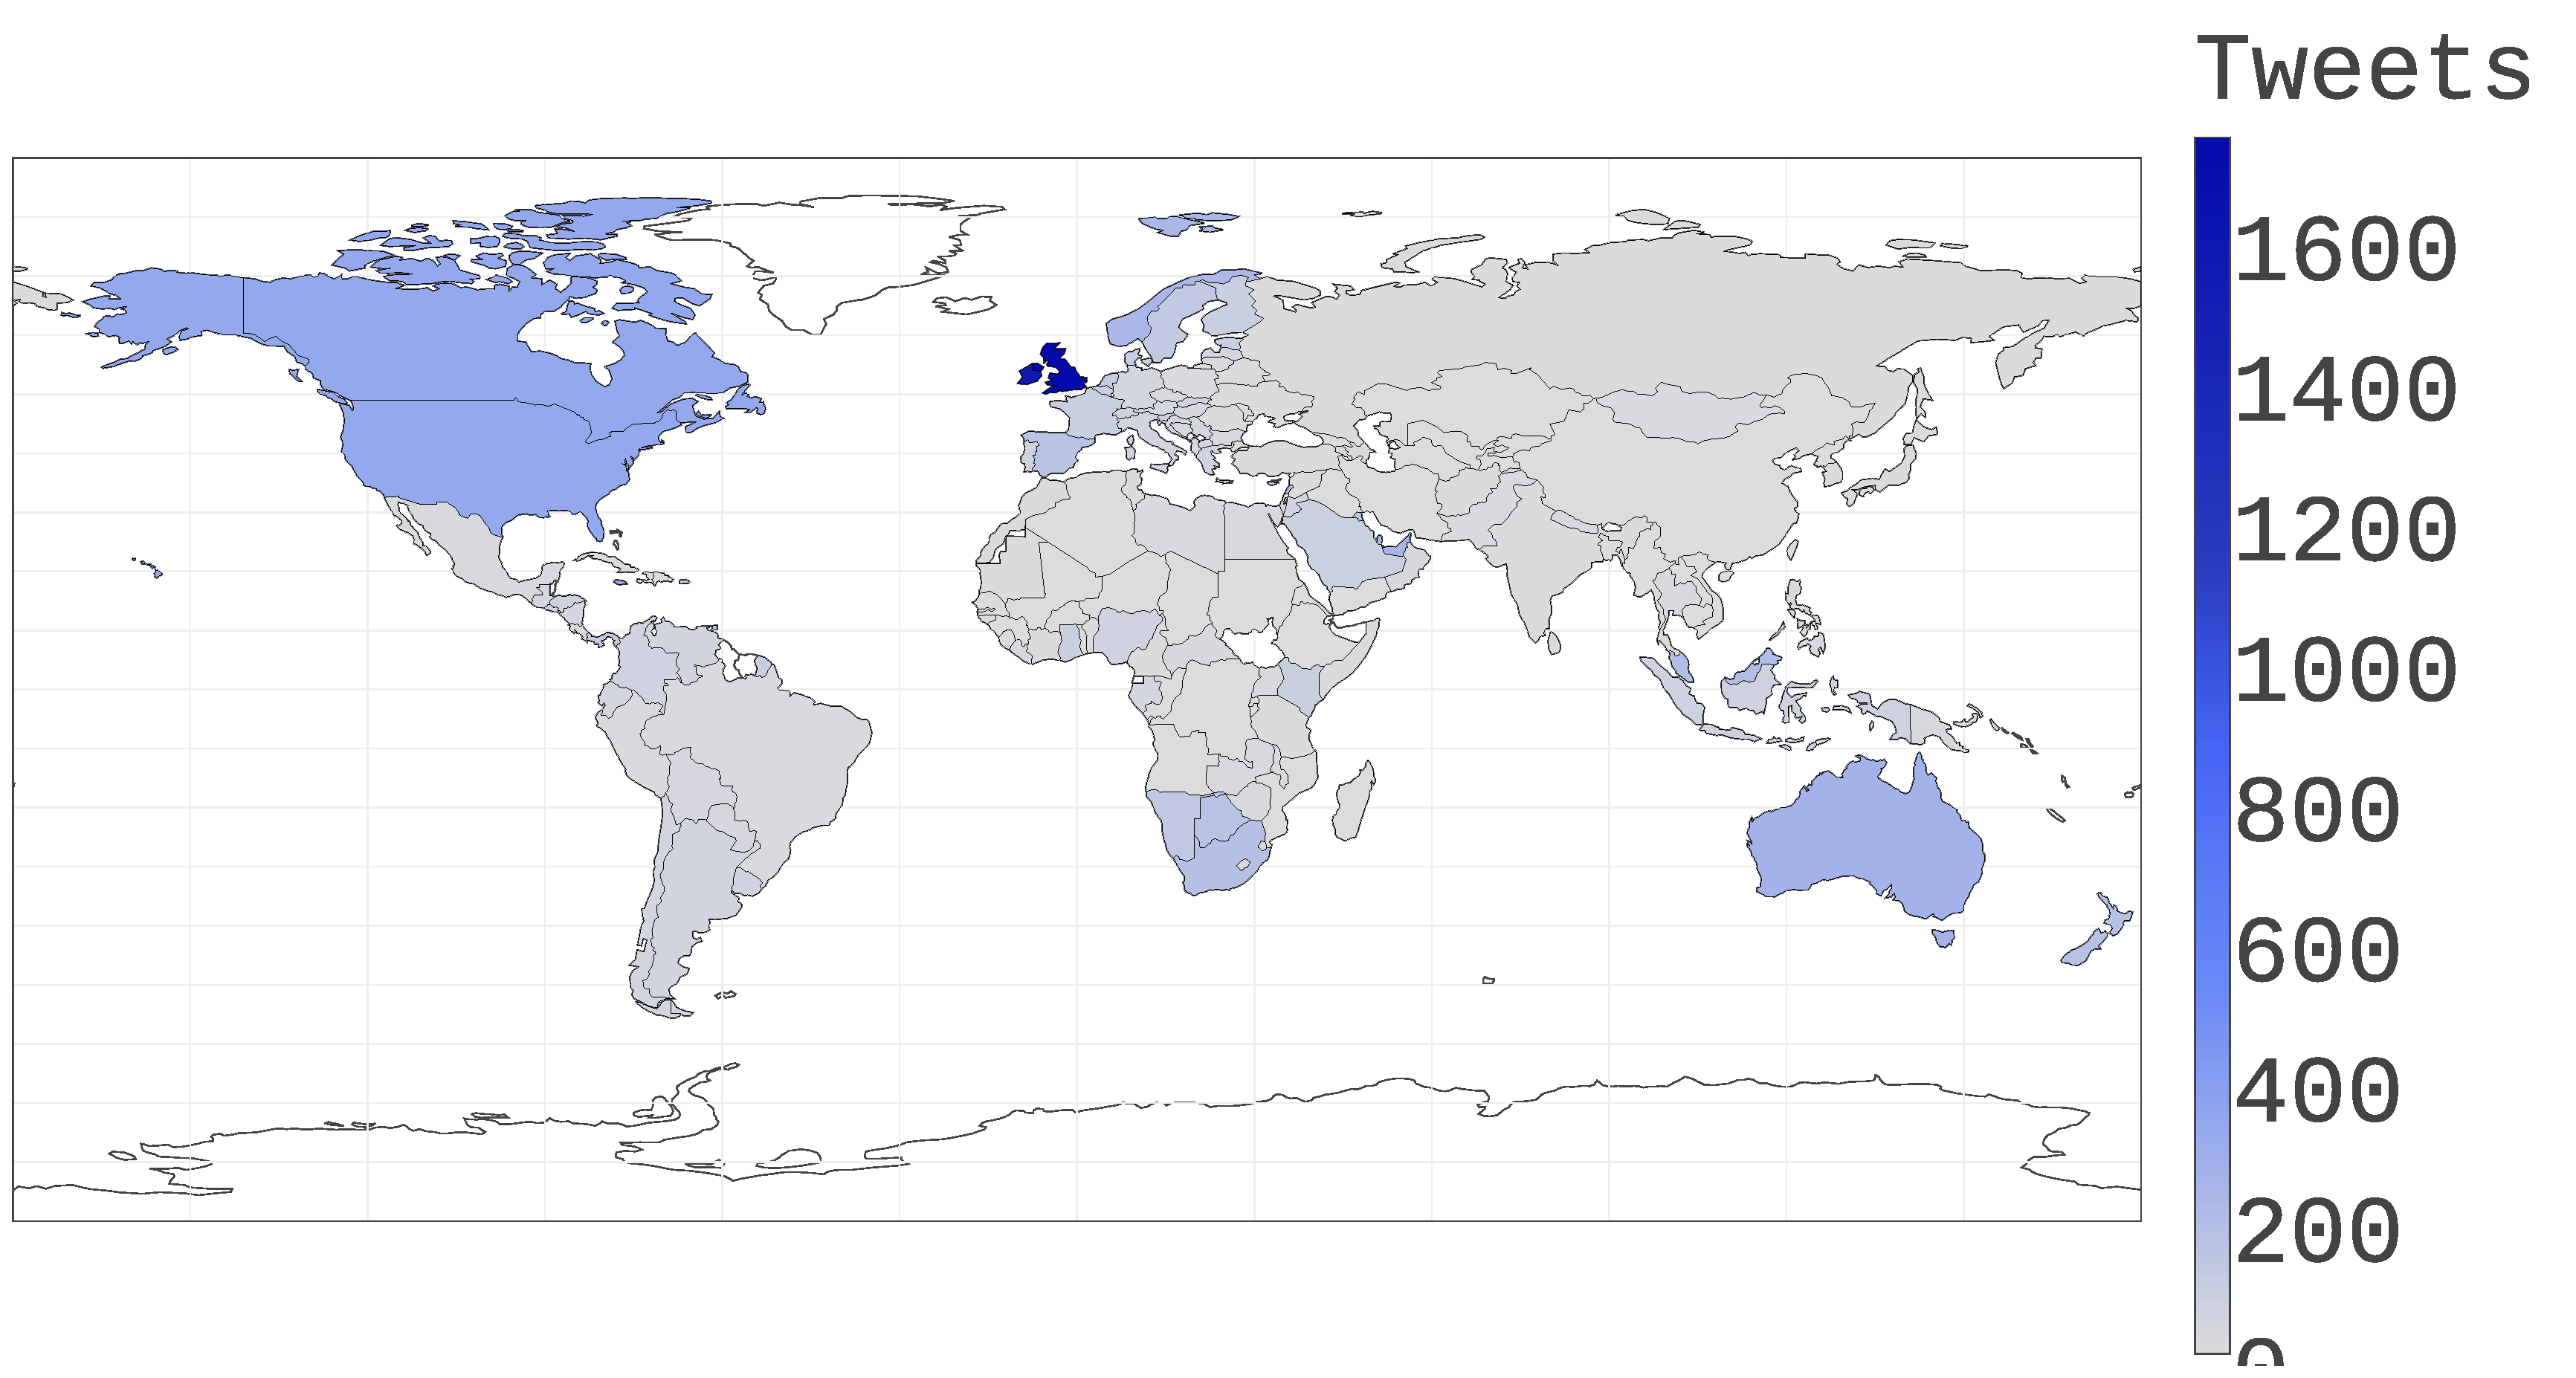
\includegraphics[width=5.3cm]{img/world/socialsensor-world-soccer_location.eps}} \\
%\vspace{-10mm}
\subfloat[Fig:][Health Epidemics]{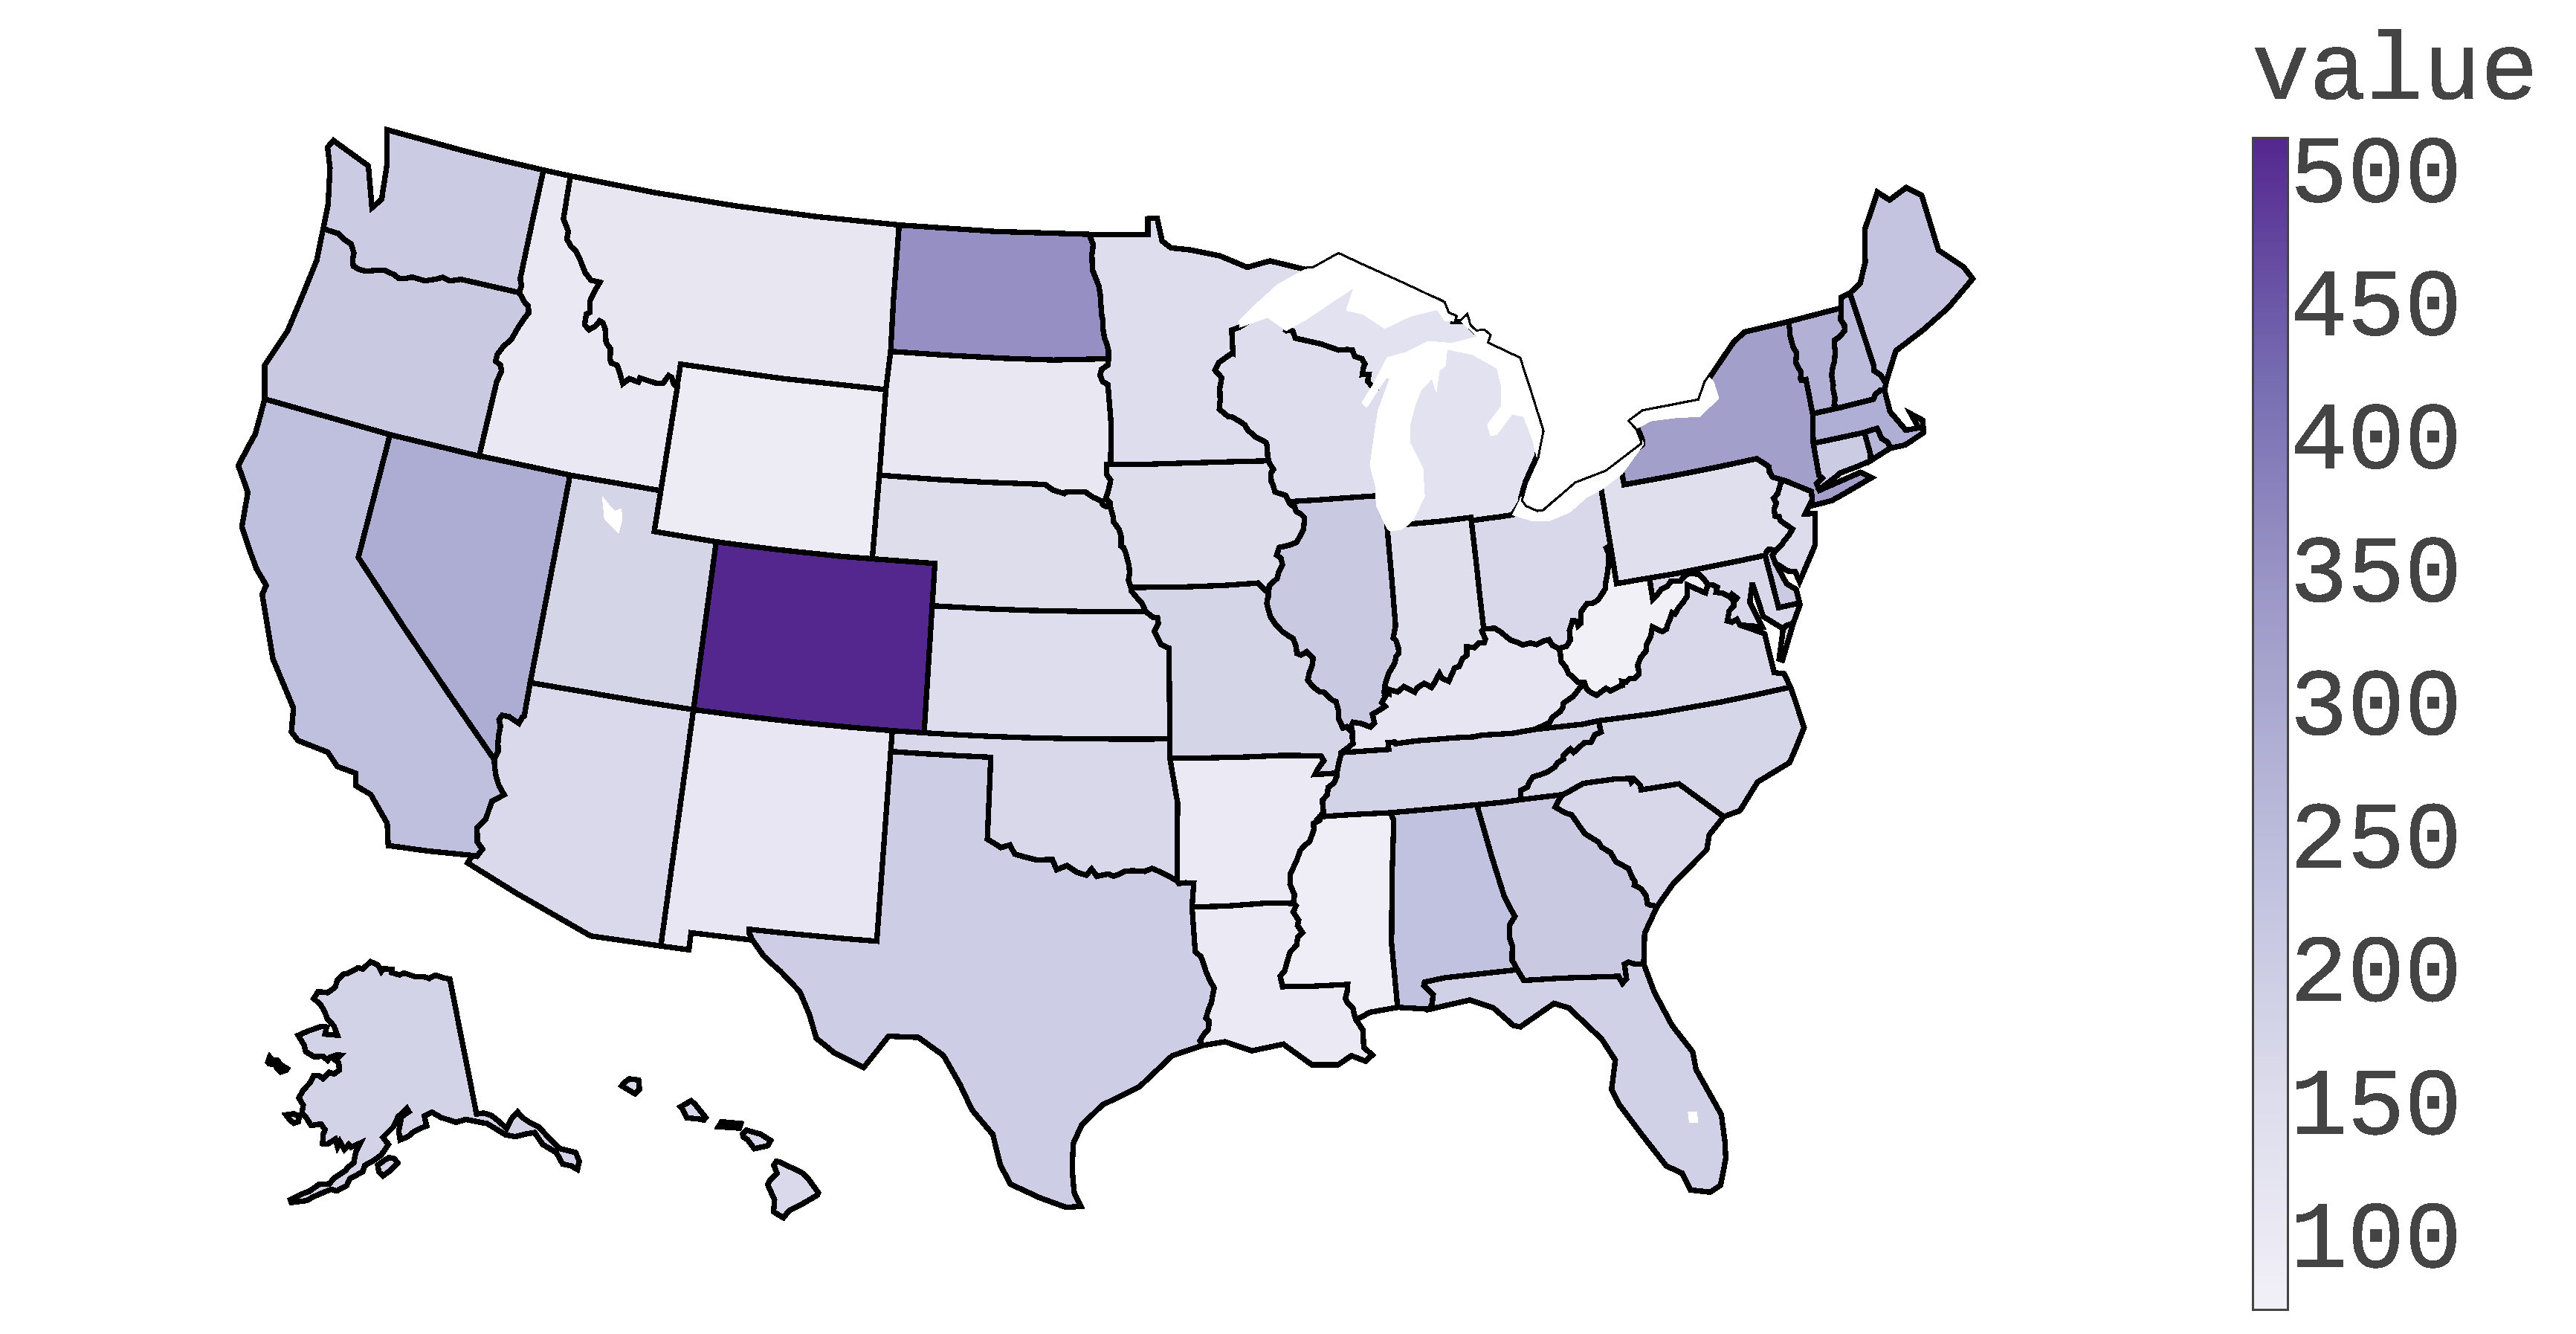
\includegraphics[width=4cm]{img/states/SocialSensor-us-states-health_epidemics_location.eps}}
\subfloat[Fig:][Social Issues]{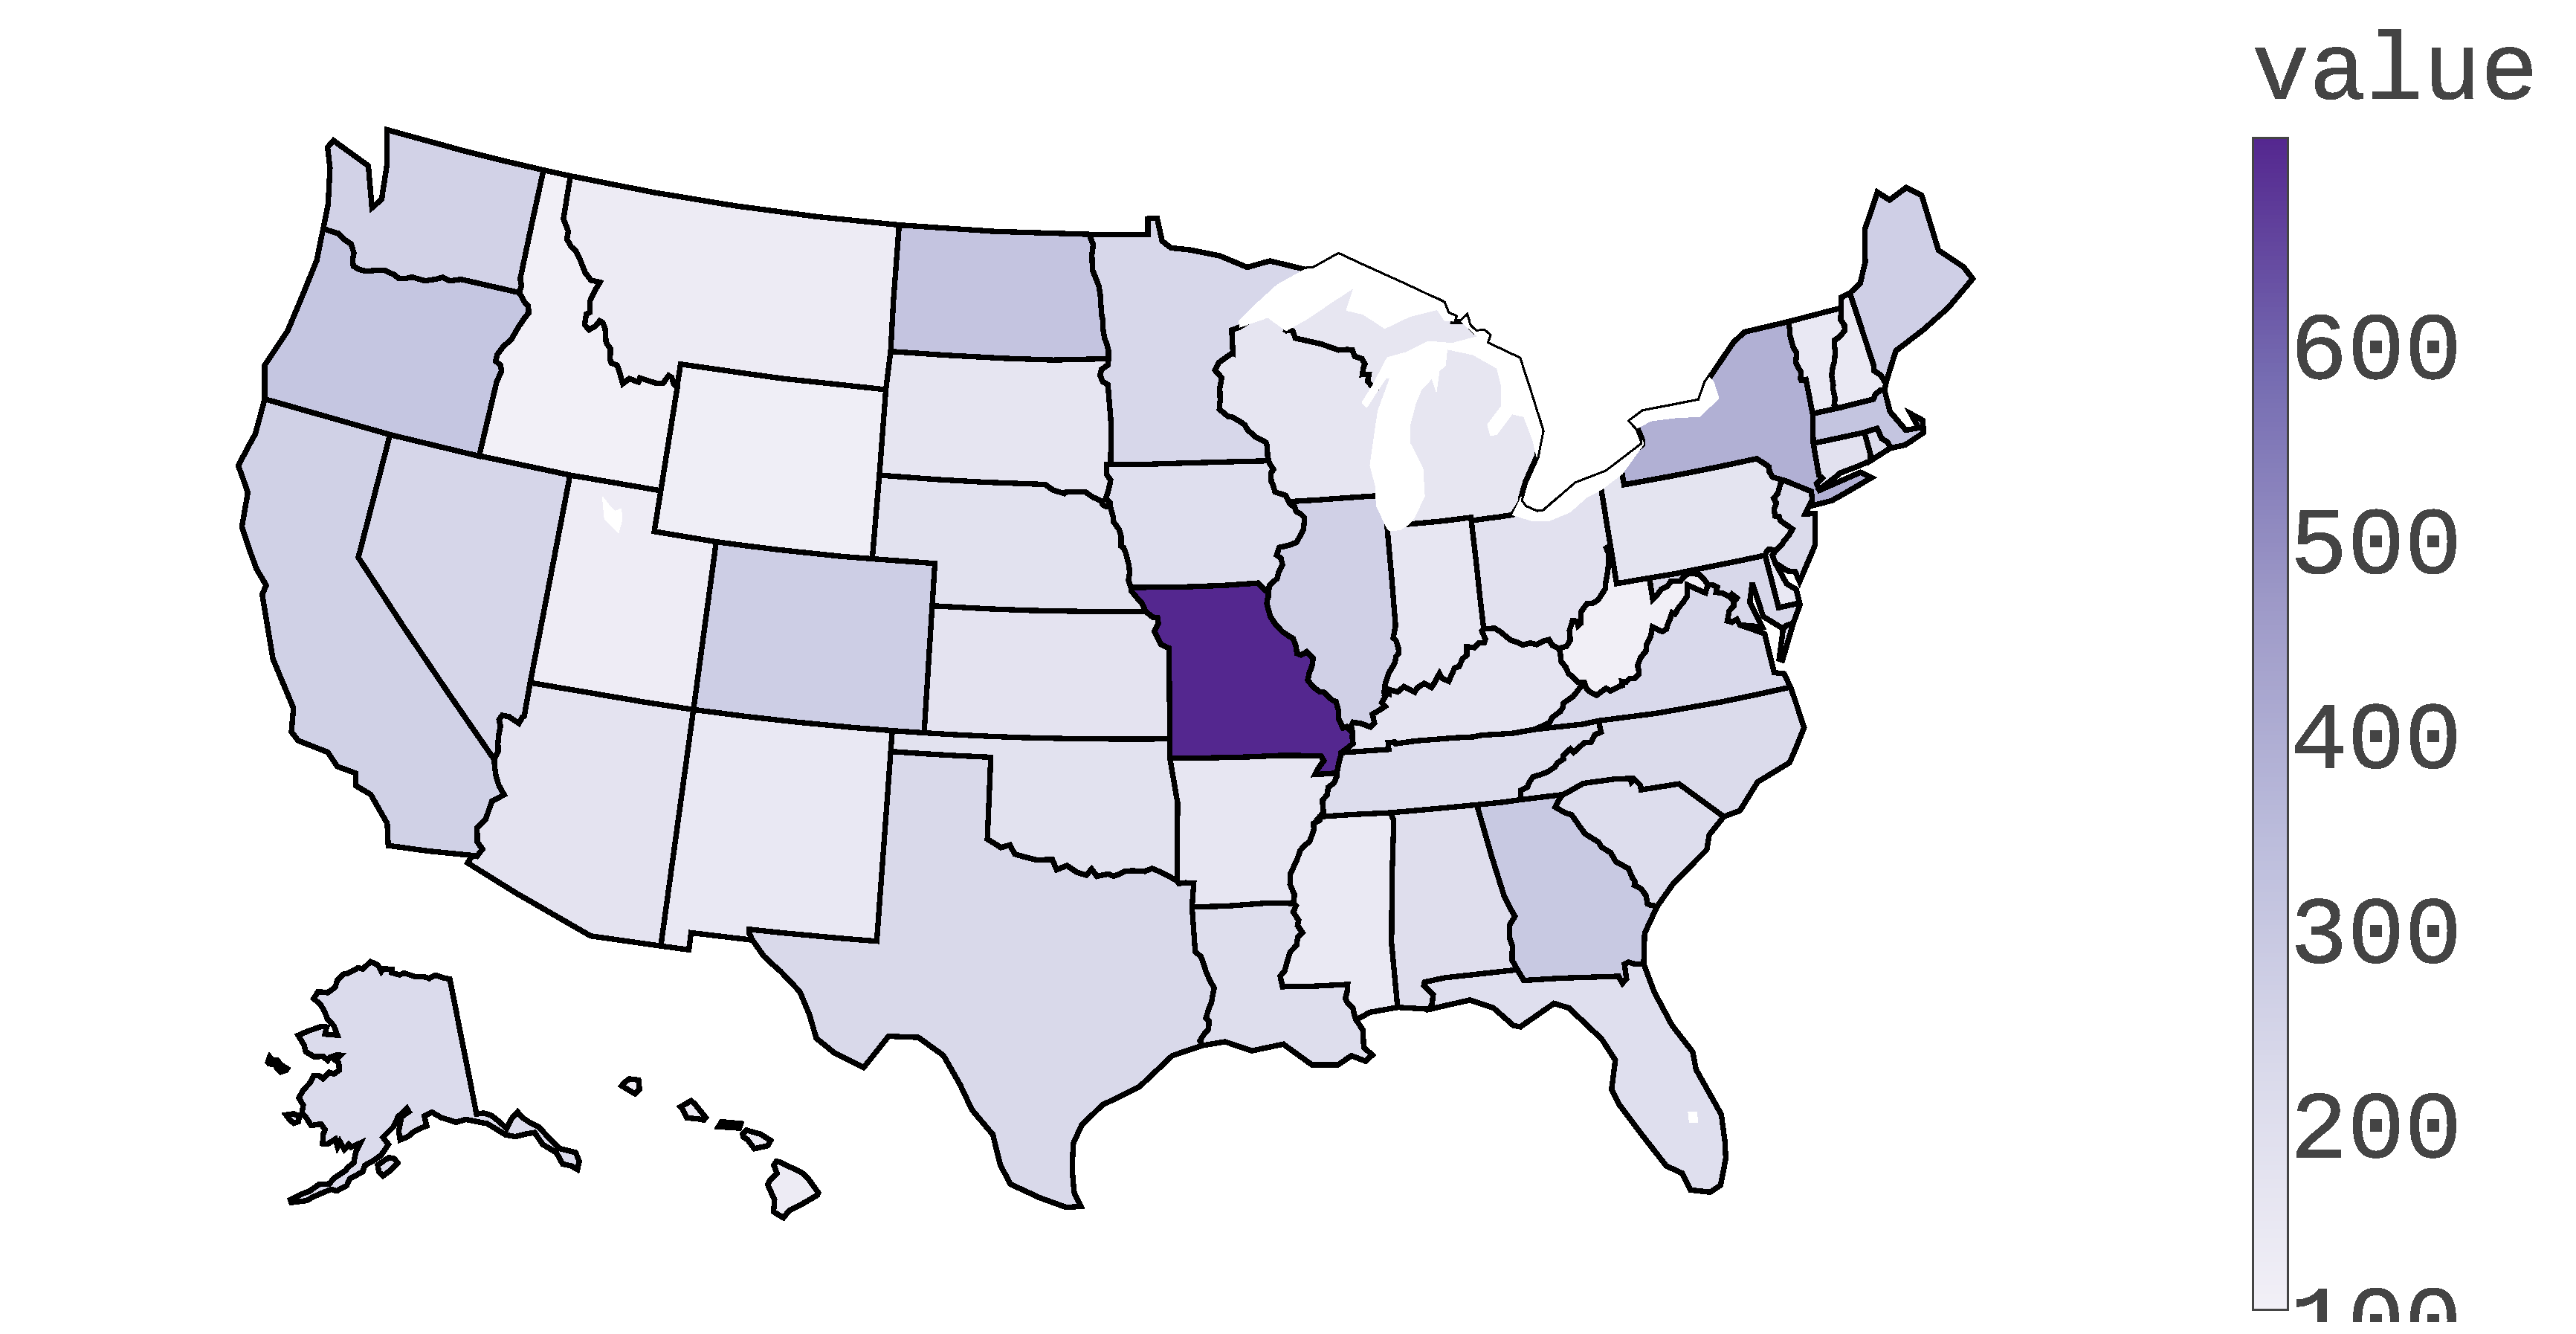
\includegraphics[width=4cm]{img/states/SocialSensor-us-states-socialissues_location.eps}}
\subfloat[Fig:][Space]{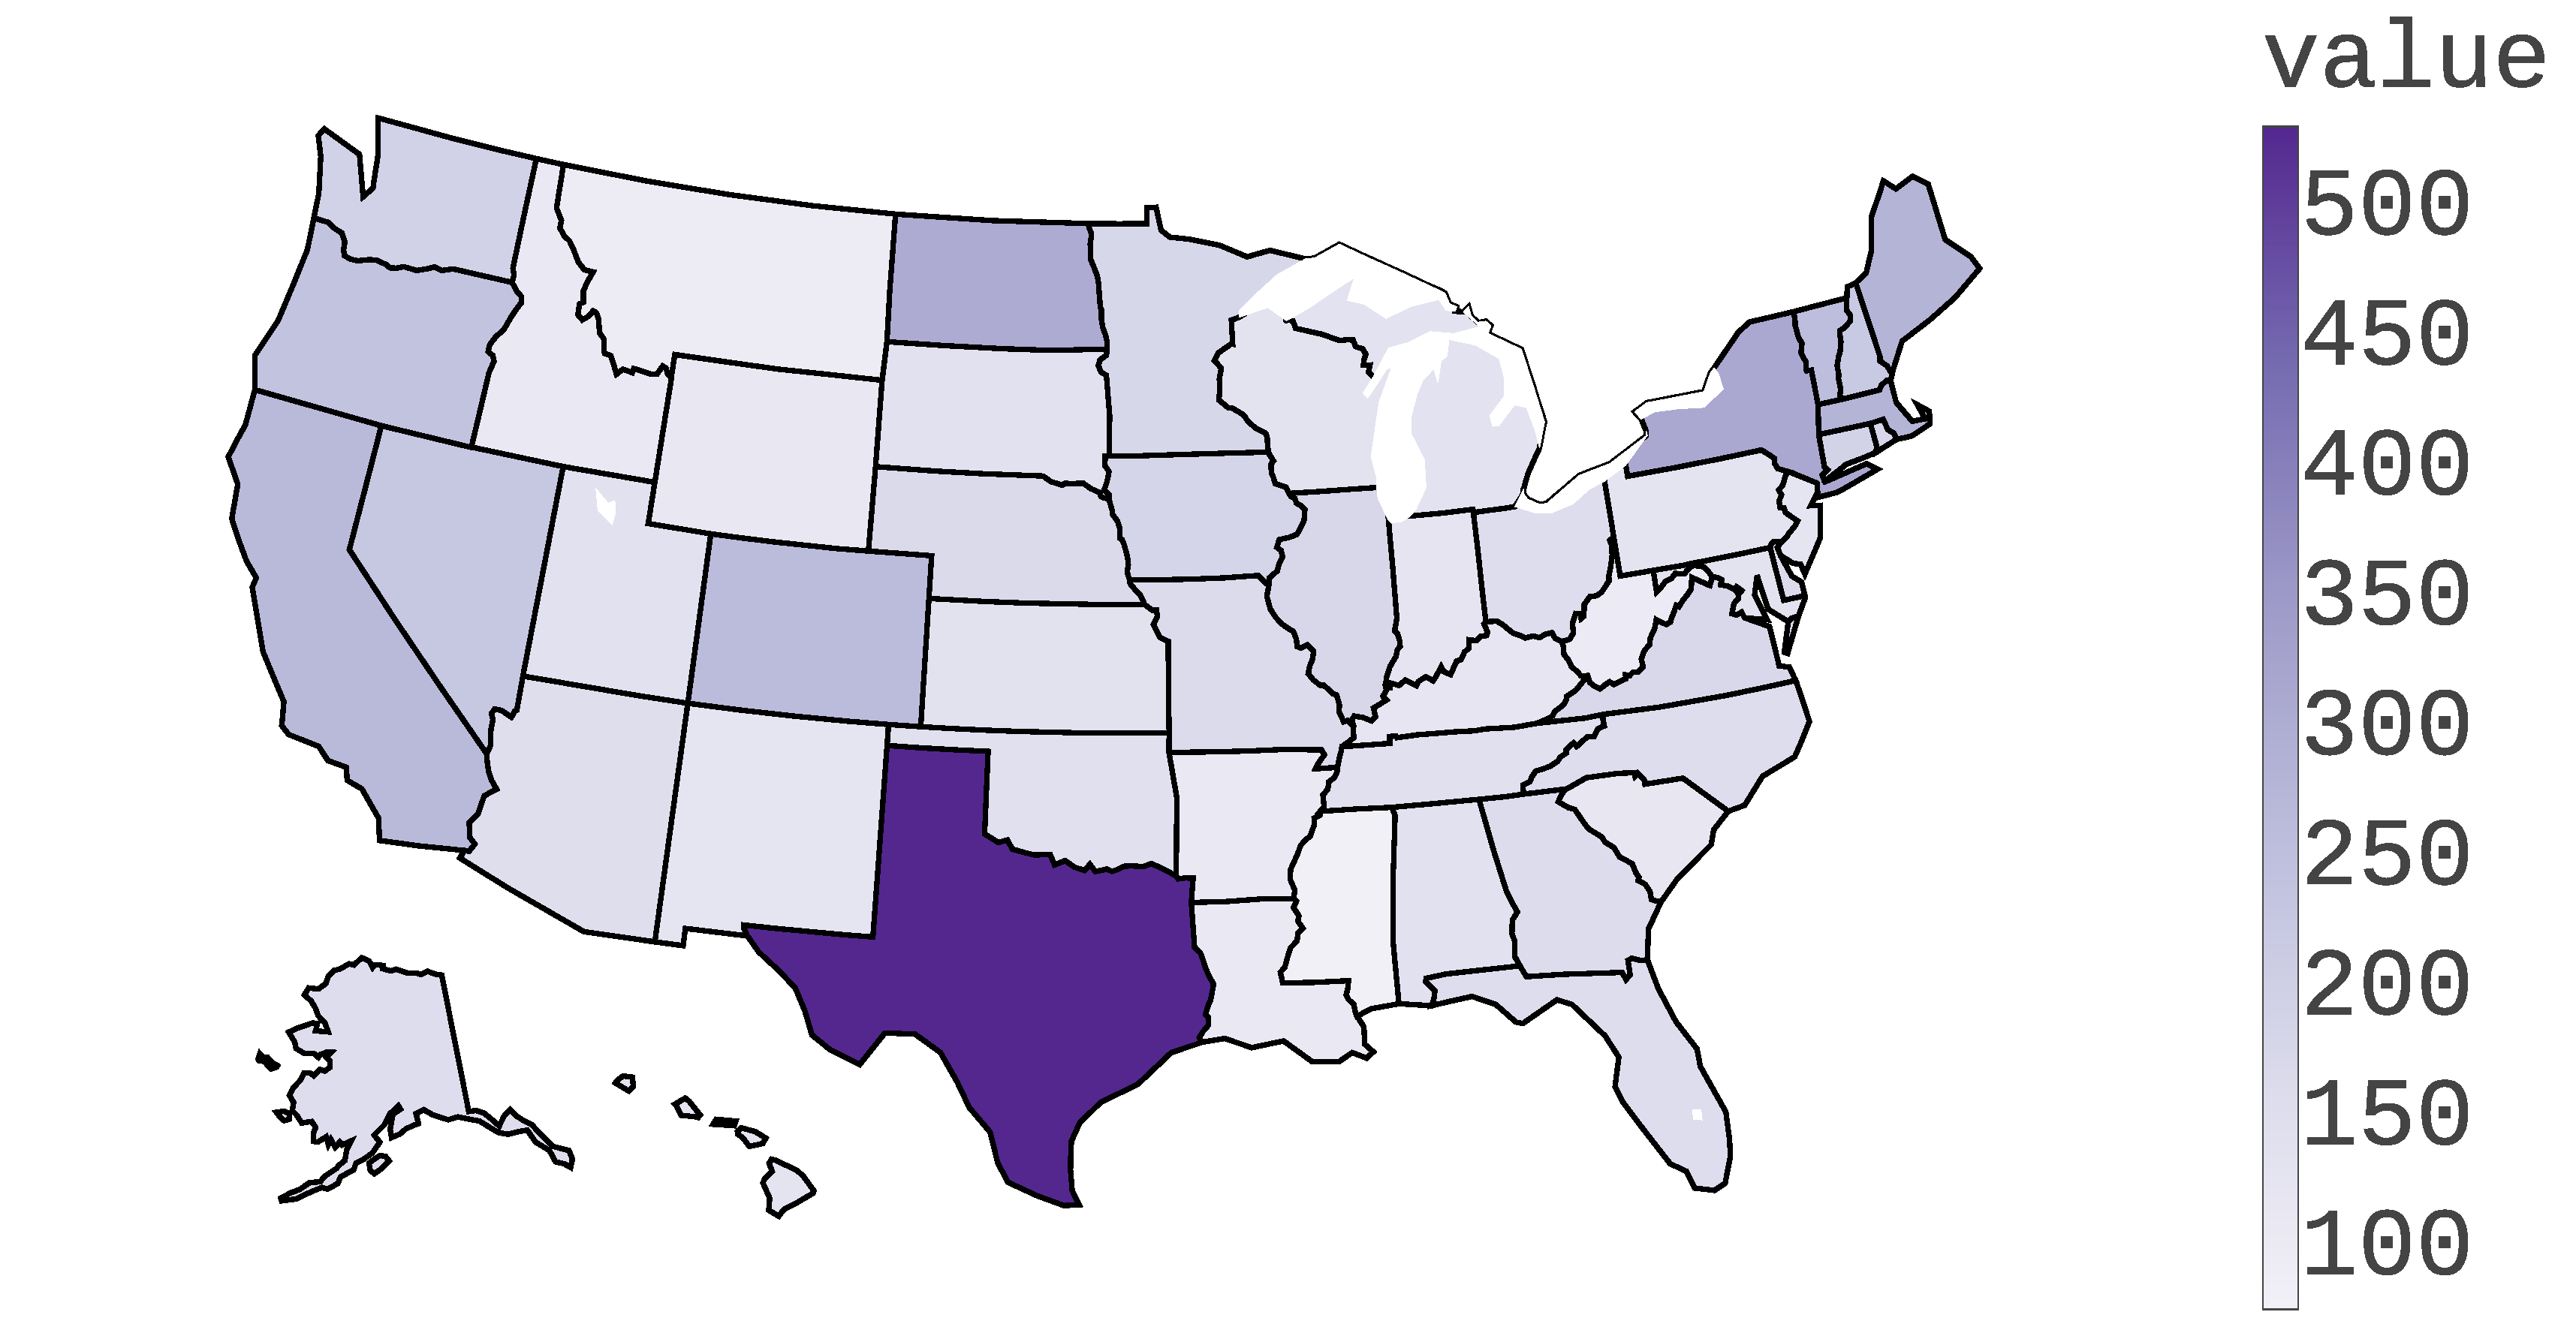
\includegraphics[width=4cm]{img/states/SocialSensor-us-states-space_location}} \\
\end{tabular}
\end{tabular}
\vspace{-2mm}
\caption {Choropleths of top: International map and bottom: U.S. map }
\label{fig:choropleths}
\end{figure*}
%%%%%%%%%%%%%%%%%%%%%%%%%%%%%%%%%%%%%%%%%%%%%%%%%%%%%%%%%%%%%%%%%%%%%%%%%%%


%%%%%%%%%%%%%%%%%%%%%%%%%%%%%%%%%%%%%%%%%%%%%%%%%%%%%%%%%%%%%%%%%%
\begin{table}[t!]
\centering
{\renewcommand{\arraystretch}{1.2}
\resizebox{0.5\textwidth}{!}{%
\begin{tabular}{|l|c|c|c|c|r|}
\hline
                                       & \multicolumn{4}{c|}{\textbf{Tweets}}                                                          & \textbf{}                           \\ \hline
\multicolumn{1}{|c|}{\textbf{Feature}} & \textbf{Max}          & \textbf{Avg}          & \textbf{Median}       & \textbf{Max entity}   & \multicolumn{1}{c|}{\textbf{Count}} \\ \hline
\textbf{From}                          & 10,196                & 8.67                  & 2                     & running\_status       & 95,547,198                          \\ \hline
\textbf{Hashtag}                       & 1,653,159             & 13.91                 & 1                     & \#retweet             & 11,183,410                          \\ \hline
\textbf{Mention}                       &                       &                       &                       &                       & 411,341,569                         \\ \hline
\textbf{Location}                      &                       &                       &                       &                       & 58,601                              \\ \hline
\textbf{Term}                          & 2024529               & 7,450.58              & 323                   & taking                & 20,234,729                          \\ \hline
\textbf{}                              & \multicolumn{4}{c|}{\textbf{Users}}                                                           &                                     \\ \hline
\textbf{From}                          & \multicolumn{1}{l|}{} & \multicolumn{1}{l|}{} & \multicolumn{1}{l|}{} & \multicolumn{1}{l|}{} &                                     \\ \hline
\textbf{Hashtag}                       & 592,363               & 10.08                 & 1                     & \#retweet             &                                     \\ \hline
\textbf{Mention}                       & 26,293                & 5.44                  & 1                     & dimensionist          &                                     \\ \hline
\textbf{Location}                      & 739,120               & 641.5                 & 2                     & london                &                                     \\ \hline
\textbf{Term}                          & 1,799,385             & 6,616.65              & 305                   & taking                &                                     \\ \hline
\textbf{}                              & \multicolumn{4}{c|}{\textbf{Hashtags}}                                                        &                                     \\ \hline
\textbf{From}                          & 18,167                & 2                     & 0                     & daily\_astrodata      &                                     \\ \hline
\end{tabular}
}}
\caption{Feature Statistics}
\label{table:featureStatistics}
\end{table}
%%%%%%%%%%%%%%%%%%%%%%%%%%%%%%%%%%%%%%%%%%%%%%%%%%%%%%%%%%%%%%%%%%

Figure \ref{fig:tweetsStats} shows details of number of tweets per month and figure \ref{fig:powerlaw} shows the power law plots of tweet counts and hashtag counts for users. We chose $10$ topics for our experiments. Tweets are temporally divided over 2 years to provide train and test sets. Table \ref{table:sampleHashtags} provides samples of training hashtags and number of train hashtags, test hashtags, topical tweets for each topic. Some topics such as $HumanCausedDisaster$ and $Soccor$ are more general topics and have higher number of topical tweets while some other ones such as $IranDeal$ is more specific, thus having less number of topical tweets.

Figure \ref{fig:locations} shows distribution of tweets across different location in U.S. and international locations overall and for each topic(?).

%%%%%%%%%%%%%%%%%%%%%%%%%%%%%%%%%%%%%%%%%%%%%%%%%%%%%%%%%%%%%%%%%%
\begin{table*}[t!]
\centering
{\renewcommand{\arraystretch}{1.2}
\resizebox{\textwidth}{!}{%
\begin{tabular}{|l|l|l|l|l|l|l|l|l|l|l|}
\hline
\textbf{Topics/Top10} & \multicolumn{1}{c|}{\textbf{NaturalDisaster}} & \multicolumn{1}{c|}{\textbf{Epidemics}} & \multicolumn{1}{c|}{\textbf{IranDeal}} & \multicolumn{1}{c|}{\textbf{SocialIssues}} & \multicolumn{1}{c|}{\textbf{LBGT}} & \multicolumn{1}{c|}{\textbf{HumanCausedDisaster}} & \multicolumn{1}{c|}{\textbf{CelebrityDeath}} & \multicolumn{1}{c|}{\textbf{Space}} & \multicolumn{1}{c|}{\textbf{Tennis}} & \multicolumn{1}{c|}{\textbf{Soccer}} \\ \hline
\textbf{\#TrainHashtags} & \multicolumn{1}{c|}{31} & \multicolumn{1}{c|}{52} & \multicolumn{1}{c|}{12} & \multicolumn{1}{c|}{31} & \multicolumn{1}{c|}{29} & \multicolumn{1}{c|}{49} & \multicolumn{1}{c|}{28} & \multicolumn{1}{c|}{98} & \multicolumn{1}{c|}{58} & 126 \\ \hline
\textbf{\#TestHashtags} & \multicolumn{1}{c|}{18} & \multicolumn{1}{c|}{33} & \multicolumn{1}{c|}{5} & \multicolumn{1}{c|}{19} & \multicolumn{1}{c|}{17} & \multicolumn{1}{c|}{29} & \multicolumn{1}{c|}{16} & \multicolumn{1}{c|}{63} & \multicolumn{1}{c|}{36} & 81 \\ \hline
\textbf{\#TotalTopicalTweets} & \multicolumn{1}{c|}{42,987} & \multicolumn{1}{c|}{210,217} & \multicolumn{1}{c|}{8,762} & \multicolumn{1}{c|}{230,058} & \multicolumn{1}{c|}{282,527} & \multicolumn{1}{c|}{408,304} & \multicolumn{1}{c|}{163,890} & \multicolumn{1}{c|}{239,719} & \multicolumn{1}{c|}{55,053} & 860,389 \\ \hline
\multirow{5}{*}{\textbf{Sample Train Hashtags}} & \#earthquake & \#ebola & \#irandeal & \#policebrutality & \#loveislove & \#gazaunderattack & \#robinwilliams & \#asteroids & \#usopenchampion & \#worldcup \\ \cline{2-11} 
 & \#storm & \#virus & \#iranfreedom & \#michaelbrown & \#gaypride & \#childrenofsyria & \#ripmandela & \#astronauts & \#novakdjokovic & \#lovesoccer \\ \cline{2-11} 
 & \#tsunami & \#vaccine & \#irantalk & \#justice4all & \#uniteblue & \#iraqwar & \#ripjoanrivers & \#satellite & \#wimbledon & \#fifa \\ \cline{2-11} 
 & \#abfloods & \#chickenpox & \#rouhani & \#freetheweed & \#homo & \#bombthreat & \#mandela & \#spacecraft & \#womenstennis & \#realmadrid \\ \cline{2-11} 
 & \#hurricanekatrina & \#theplague & \#nuclearpower & \#newnjgunlaw & \#gaymarriage & \#isis & \#paulwalker & \#telescope & \#tennisnews & \#beckham \\ \hline
\end{tabular}
}
}
\caption{Test/Train Hashtag samples and statistics}
\label{table:sampleHashtags}
\end{table*}
%%%%%%%%%%%%%%%%%%%%%%%%%%%%%%%%%%%%%%%%%%%%%%%%%%%%%%%%%%%%%%%%%%


\section{Experimental Methodology}

How we curated hashtags: need to make up good story here.  Inner-annotator agreement of 3/4.

Train/validation/test split date selection -- temporally .5,.1,.4

Feature selection: threshold per feature 159 and 50 (just explain rationale for lower hashtag and location thresholds).

Formal notation, how do we train/test and tune hyperparameters for a generic classifier.

\subsection{Classification Algorithms}

\begin{enumerate}
\item Naive Bayes
\item Rocchio (centroid)
\item Logistic Regression
\end{enumerate}

All above over 1,000,000 features, *same* training data for all algorithms.

Not breaking down by feature type yet -- that's for the feature analysis section.

\subsection{Analysis}

- Table of rows:alg, cols: MAP, P@k (k in {10,100,1000}) with stderrs over all topics

- Could do a bar graph (below) each for MAP, P@100 with topics as major columns and algs as neighboring bars

- Anecdotal results for each topic -- point out deficiency in our labels (a good thing, we generalized well from small hashtag set), manual evaluation of relevance for top-100 for best algorithm?

%%%%%%%%%%%%%%%%%%%%%%%%%%%%%%%%%%%%%%%%%%%%%%%%%%%%%%%%%%%%%%%%%%
\begin{table*}[t]
\centering
{\renewcommand{\arraystretch}{1.2}
\resizebox{\textwidth}{!}{%
\begin{tabular}{|l|l|c|c|c|c|c|c|c|c|c|c|c|}
\hline
\textbf{Method} & \textbf{Metric} & \textbf{Tennis} & \textbf{Space} & \textbf{Soccer} & \textbf{IranDeal} & \textbf{HumanCausedDisaster} & \textbf{CelebrityDeath} & \textbf{SocialIssues} & \textbf{NaturalDisaster} & \textbf{Epidemics} & \textbf{LGBT} & \textbf{Mean$\pm$Std} \\ \hline
\textbf{LR} & \textbf{MAP} & 0.918 & 0.870 & 0.827 & 0.811 & 0.761 & 0.719 & 0.498 & 0.338 & 0.329 & 0.165 & 0.623$\pm$0.19 \\ \hline
\textbf{NB} & \textbf{MAP} & 0.908 & 0.897 & 0.731 & 0.824 & 0.785 & 0.748 & 0.623 & 0.267 & 0.178 & 0.092 & 0.605$\pm$0.22 \\ \hline
\textbf{Rocchio} & \textbf{MAP} & 0.690 & 0.221 & 0.899 & 0.584 & 0.481 & 0.253 & 0.393 & 0.210 & 0.255 & 0.089 & 0.407$\pm$0.18 \\ \hline
\textbf{RankSVM} & \textbf{MAP} & 0.702 & 0.840 & 0.674 & 0.586 & 0.603 & 0.469 & 0.370 & 0.248 & 0.136 & 0.082 & 0.471$\pm$0.18 \\ \hline \hline
\textbf{LR} & \textbf{P@10} & 1.000 & 0.000 & 0.200 & 0.700 & 0.600 & 0.000 & 0.100 & 0.200 & 0.300 & 0.500 & 0.360$\pm$0.24 \\ \hline
\textbf{NB} & \textbf{P@10} & 1.000 & 0.900 & 0.700 & 0.600 & 0.600 & 0.700 & 1.000 & 0.100 & 0.400 & 0.100 & 0.610$\pm$0.23 \\ \hline
\textbf{Rocchio} & \textbf{P@10} & 0.800 & 0.000 & 1.000 & 0.900 & 0.000 & 0.000 & 0.000 & 0.500 & 0.500 & 0.100 & 0.380$\pm$0.29 \\ \hline
\textbf{RankSVM} & \textbf{P@10} & 1.000 & 0.800 & 0.600 & 0.800 & 0.400 & 0.300 & 0.000 & 0.100 & 0.000 & 0.200 & 0.420$\pm$0.26 \\ \hline \hline
\textbf{LR} & \textbf{P@100} & 0.950 & 0.580 & 0.650 & 0.870 & 0.620 & 0.490 & 0.640 & 0.690 & 0.790 & 0.210 & 0.649$\pm$0.15 \\ \hline
\textbf{NB} & \textbf{P@100} & 0.980 & 0.850 & 0.600 & 0.880 & 0.750 & 0.860 & 0.730 & 0.230 & 0.090 & 0.190 & 0.616$\pm$0.23 \\ \hline
\textbf{Rocchio} & \textbf{P@100} & 0.980 & 0.000 & 1.000 & 0.690 & 0.170 & 0.000 & 0.280 & 0.170 & 0.680 & 0.120 & 0.409$\pm$0.28 \\ \hline
\textbf{RankSVM} & \textbf{P@100} & 0.730 & 0.720 & 0.310 & 0.700 & 0.880 & 0.440 & 0.480 & 0.340 & 0.020 & 0.100 & 0.472$\pm$0.20 \\ \hline \hline
\textbf{LR} & \textbf{P@1000} & 0.963 & 0.954 & 0.816 & 0.218 & 0.899 & 0.833 & 0.215 & 0.192 & 0.343 & 0.071 & 0.550$\pm$0.26 \\ \hline
\textbf{NB} & \textbf{P@1000} & 0.954 & 0.954 & 0.716 & 0.218 & 0.904 & 0.881 & 0.215 & 0.195 & 0.141 & 0.060 & 0.524$\pm$0.28 \\ \hline
\textbf{Rocchio} & \textbf{P@1000} & 0.604 & 0.000 & 0.925 & 0.218 & 0.359 & 0.000 & 0.215 & 0.167 & 0.144 & 0.065 & 0.270$\pm$0.21 \\ \hline
\textbf{RankSVM} & \textbf{P@1000} & 0.799 & 0.922 & 0.764 & 0.218 & 0.525 & 0.547 & 0.215 & 0.173 & 0.154 & 0.064 & 0.438$\pm$0.22 \\ \hline
\end{tabular}
}}
\caption{Different learning methods results on topics with hyper-parameter tuning based on MAP}
\label{table:results2}
\end{table*}
%%%%%%%%%%%%%%%%%%%%%%%%%%%%%%%%%%%%%%%%%%%%%%%%%%%%%%%%%%%%%%%%%%

%%%%%%%%%%%%%%%%%%%%%%%%%%%%%%%%%%%%%%%%%%%%%%%%%%%%%%%%%%%%%%%%%%
\begin{table*}[]
\large
{\renewcommand{\arraystretch}{1.2}
\resizebox{\textwidth}{!}{
\begin{tabular}{|l|l|}
\hline
\textbf{Tennis} & \textbf{Space} \\ \hline 
\checkmark rt @espntennis: shock city. darcis drops rafa in straight sets. first time nadal loses in first rd of a. major in career. \#espnwimbledon \#wÉ & \xmark  rt @jaredleto: rt @30secondstomars: icymi: mars performing a cover of @rihanna's \#stay on australia's @triplemmelb - video \_ http://t.co/uqÉ \\ \hline
\checkmark rt @espntennis: shock city. darcis drops rafa in straight sets. first time nadal loses in first rd of a. major in career. \#espnwimbledon \#wÉ & \xmark  voting mars @30secondstomars @jaredleto @shannonleto @tomofromearth xobest group http://t.co/dlsozvjinf \\ \hline
\checkmark rt @espntennis: shock city. darcis drops rafa in straight sets. first time nadal loses in first rd of a. major in career. \#espnwimbledon \#wÉ & \xmark  rt @jaredleto\_com: show everyone how much you are proud of @30secondstomars !\#mtvhottest 30 seconds to mars http://t.co/byxnri4t67 \\ \hline
\checkmark rt @espntennis: shock city. darcis drops rafa in straight sets. first time nadal loses in first rd of a. major in career. \#espnwimbledon \#wÉ & \xmark  rt @30secondstomars: missed the big news? mars touring with @linkinpark + special guests @afi this summer!\_ http://t.co/3e5rm9pwrd \\ \hline
\checkmark rt @espntennis: shock city. darcis drops rafa in straight sets. first time nadal loses in first rd of a. major in career. \#espnwimbledon \#wÉ & \xmark  rt @30secondstomars: to the right,to the left,we will fightto the death.go \#intothewildonvyrt with mars, starting weekly, nov 30 \_ httÉ \\ \hline
\textbf{Soccer} & \textbf{IranDeal} \\ \hline
\xmark  rt @tomm\_dogg: \#thingstodobeforeearthends spend all my money. & \checkmark rt @iran\_policy: @vidalquadras:@isjcommittee has investigated 10 major subjects of iranŐs controversial \#nuclear program \#irantalksvienna \\ \hline
\starmark  @mancityonlineco nice performance & \checkmark rt @iran\_policy: @vidalquadras:@isjcommittee has investigated 10 major subjects of iranŐs controversial \#nuclear program \#irantalksvienna \\ \hline
\starmark  rt @indykaila: podolski: "let's see what happens in the winter. the fact is that i'm not happy with it, that's clear." @arsenal & \xmark  rt @negarmortazavi: thank you @hassanrouhani for retweeting. let's hope for a day when no iranian fears returning to their homeland. http:/É \\ \hline
\starmark  rt @indykaila: wenger: "i don't believe match-fixing is a problem in england." \#afc & \xmark  rt @iran\_policy: iran: details of savage attack on political prisoners in evin prison http://t.co/xdzuakqdiv \#iran \#humanrights \\ \hline
\xmark  @indykaila you never got back to me about tennis this week & \checkmark rt @iran\_policy: chairman ros-lehtinen speaking on us commitment 2 protect camp liberty residents. \#iranhrviolations http://t.co/1g6dhx1znu \\ \hline
\textbf{HumanCausedDisaster} & \textbf{CelebrityDeath} \\ \hline
\checkmark rt @baselsyrian: there`ve been peaceful people in \#homs not terrorists! \#assad,enemy of \#humanity destroyed it. \#eyeonhoms \#withsyria http:É & \starmark  rt @sawubona\_chris: today is my birthday \&amp; also the day my hero @nelsonmandela has died. lets never forget what he taught us. forgiveness iÉ \\ \hline
\checkmark what a helpless father, he can do nothing under \#assad's siege!\#speakup4syrianchildren  http://t.co/vgle3byebw\#syria \#syriawarcrimes \#un & \starmark  rt @nelsonmandela: Ňdeath is something inevitable.when a man has done what he considers to be his duty to his people\&amp;his country,he can resÉ \\ \hline
\starmark  exclusive: us formally requested \#un investigation; russia pressured \#assad to no avail;chain of evidence proof hard http://t.co/560t2rvdfw & \starmark  rt @nelsonmandela: la muerte es algo inevitable.cuando un hombre ha hecho lo que considera que es su deber para con su gente y su pa’s,puedÉ \\ \hline
\starmark  \#save\_aleppo from \#assadwarcrimes\#save\_aleppo from \#civilians -targeted shelling of \#assad regime\#syria \#aleppo http://t.co/k3dfxh0pxl & \xmark   \#jacques \#kallis: a phenomenal cricketing giant of all time - \#cricket \#history \#southafrica http://t.co/ms5pmwoag9 \\ \hline
\checkmark rt @canine\_rights: why does the \#un allow this to continue? rt@tintin1957 help raise awareness of the suffering in \#syriawarcrimes http://tÉ & \xmark  @sudesh1304 south africa has the most beautiful babies....so diverse,so unique...so god!! lol \#durban \#southafrica \\ \hline
\textbf{SociallIssues} & \textbf{NaturalDisaster} \\ \hline
\starmark  the us doesn't actually borrow is the thing. i believe in a creationist theory of the us dollar @usanationdebt @nationaldebt & \xmark  us execution in \#oklahoma :  not cruel and unusual?  maybe just barbaric, inhumane and reminiscent of the dark ages! \\ \hline
\starmark  rt @2anow: according to @njsenatepres women's rights do not include this poor nj mother's right to defend herself http://t.co/xzbslnqkh6  \#É & \xmark  \#haiti \#politics - the haiti-dominican crisis - i agree with how martelly is handling the situation: i totally... http://t.co/ro4pswsszs \\ \hline
\starmark  rt @2anow: confiscation ? how many carry permits are in the senate and assembly? give us ours or turn them in.  @senatorlorettaw @lougreenwÉ & \starmark  rt @soilhaiti: a new reforestation effort in \#haiti. local compost, anyone? http://t.co/xpad0rqbjk @richardbranson @clintonfdn @virginuniteÉ \\ \hline
\starmark  rt @2anow: vote with your wallet against \#guncontrolforest city enterprises does not support the \#2a http://t.co/tpkok3berm\#nj2as  \#tcot & \xmark  mes cousins jamais nŽs hantent les nuits de duvalier \#haiti \#duvalier \\ \hline
\starmark  @2anow @momsdemand @jstines3 they dont have a plan for that , which is why they should never be allowed to take our guns & \checkmark tony burgener of @swisssolidarity says you can't compare the disaster response in \#haiti with the response to \#haiyan in \#philippines @iheid \\ \hline
\textbf{Epidemics} & \textbf{LGBT} \\ \hline
\checkmark rt @who: fourteen of the susp. \&amp; conf. ebola cases in \#conakry, \#guinea, are health care workers, of which 11 died \#askebola & \starmark  rt @jackmcoldcuts: @lunaticrex @fingersmalloy @toddkincannon @theanonliberal anthony kennedy just wrote opinion granting legal protection to cupcake kiplers \\ \hline
\xmark  @who who can afford also been cover in government health insurance {[}with universal health coverage{]} & \xmark  @toddkincannon your personal account, your interest. separate from your business. \\ \hline
\checkmark \#ebolaoutbreak this health crisis..unparalleled in modern times,Ó @who dir. aylward - requires \$1 billion to stem http://t.co/rjzqhydb3d & \xmark  why would you report someone as spam if he is not spam? @illygirlbrea @toddkincannon \\ \hline
\xmark  rt @medsin: @who are conducting a survey on the social determinants of health in medical teaching. fill the survey in at https://t.co/aj59xÉ & \xmark  rt @t3h\_arch3r: @toddkincannon thanks for your tl having the female realbrother. between them is 600 lbs. 104 iq points. and a lot of hate. \\ \hline
\xmark  augmentation vertigineuse de 57,4\% en 1 an des actes islamophobes en france, dit le collectif contre l'islamophobie http://t.co/2qjhocegi5 & \xmark  @toddkincannon who us dick trickle. \\ \hline
\end{tabular}
}
}
\caption{Top Tweets for each topic based on MAP tuned results}
\label{table:topTweets}
\end{table*}
%%%%%%%%%%%%%%%%%%%%%%%%%%%%%%%%%%%%%%%%%%%%%%%%%%%%%%%%%%%%%%%%%%

\section{Feature Analysis}

%\textbf{What we have to work with: topics, features, feature attributes}
In this section, we analyze the informativeness of each feature for learning topical tweets by looking at different characteristics for each feature in our dataset. For example, one characteristic of hashtags could be the number of the tweets that contain those hashtags. Does this have an effect on importance of the hashtag when it comes to learning topical tweets or not. In this sense, this section would bring insights to the following questions:

\begin{itemize}
\item \textbf{What are the best features for learning social sensors, do they differ by topic?  (Why?)}
\item \textbf{For each feature type, do any attributes correlate with importance?}
\end{itemize}

A famous method for measuring informativeness is Mutual Information which is a measure of amount of information one random variable contains about another random variable. In order to calculate amount of information that a feature $f_k \in \{from, hashtag, mention, term, location\}$ provides w.r.t $t_i \in \{NaturalDisaster, Epidemics, ...\}$, mutual information is defined as:

\begin{multline}
I(t_i, f_k)= \\
 \sum_{t_i\in \{ true, false \}} \sum_{f_k\in \{ true, false\}}p(f_k,t_i)\log \left ( \frac{p(f_k,t_i)}{p(f_k)p(t_i)} \right )
 \label{eq:eq1}
\end{multline}

Higher values for this metric indicates more informative features for the specified topic.

First, we provide mutual information values for each feature across different topics shown by boxplots in figure \ref{fig:miboxplots}, and average values of mutual information for each feature vs different topics shown in table \ref{fig:table1}. The last column in table \ref{fig:table1} shows average mutual information for the feature with the standard error range provided. We make a few observations from the analysis of Table \ref{fig:table1}:

\begin{itemize}
\item Term features provide more information for all of the topics on average which shows the importance of uni-grams when it comes to selection of topical tweet.
\item From and mention features are the least informative features for all of the topics.
\item Location and Hashtag feature provide second and third most informative features respectively.
\item A few topics such as irandeal and tennis are less sensitive to selection of a specific features.
\item Location feature provides more information regarding HumanCausedDisaster, LBGT, and Soccer topics.
\item Sorting features based on their average mean value across different topics results in the following order:
\begin{enumerate}
\item Term
\item Location
\item Hashtag
\item Mention
\item From
\end{enumerate}
\end{itemize}

%%%%%%%%%%%%%%%%%%%%%%%%%%%%%%%%%%%%%%%%%%%%%%%%%%%%%%%%%%%%%%%%%%%%%%%%%%%
\iffalse
\begin{figure}[tbph!]
\centering
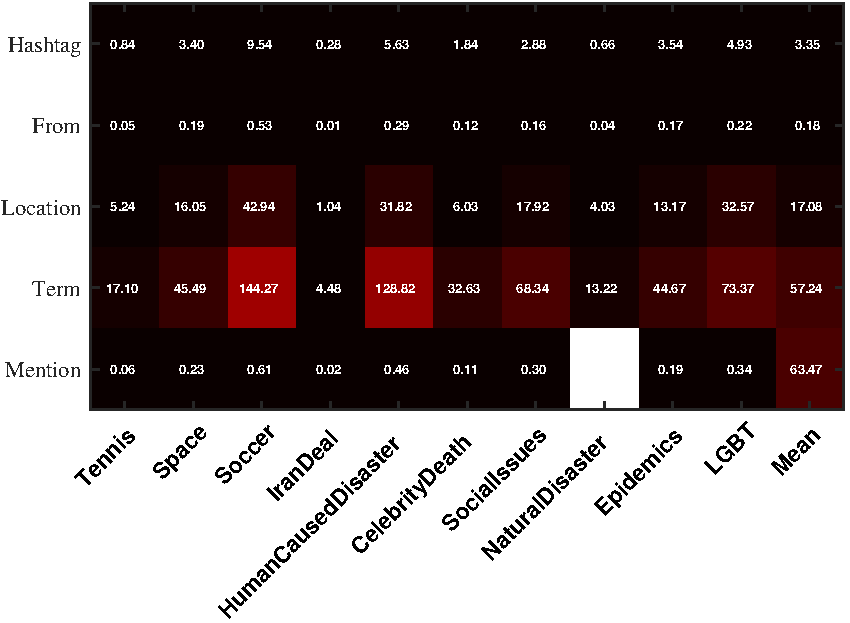
\includegraphics[width=0.5\textwidth]{images/avgMI.pdf}
\vspace{-3mm}
\caption{Average MI for different features vs. Topics, last two column show mean value and stderr across all topics}
\label{fig:table1}
\end{figure}

\begin{figure}[h!]
\centering
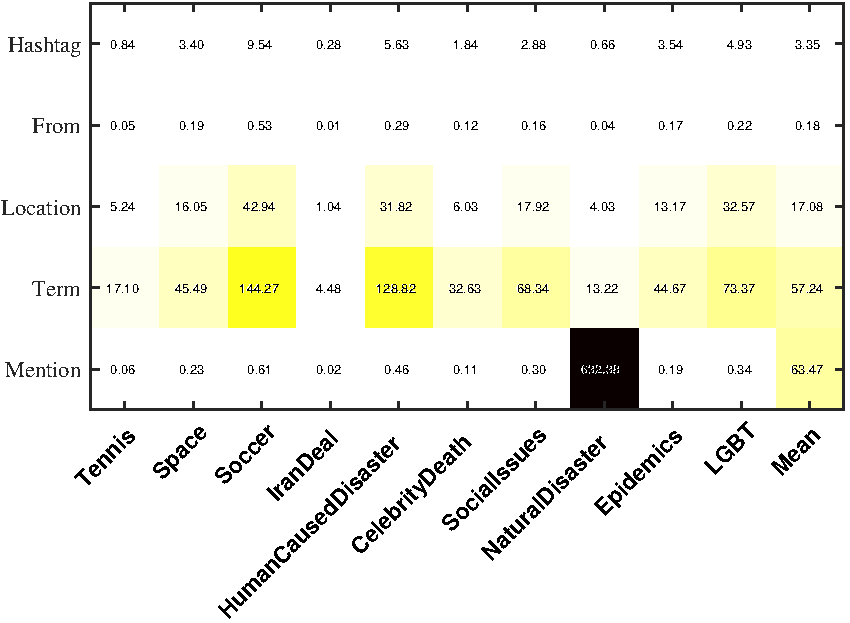
\includegraphics[width=0.5\textwidth]{images/avgMI2.pdf}
\vspace{-3mm}
\caption{Average MI for different features vs. Topics, last two column show mean value and stderr across all topics}
\label{fig:table1}
\end{figure}
\fi
\begin{figure}[h!]
\centering
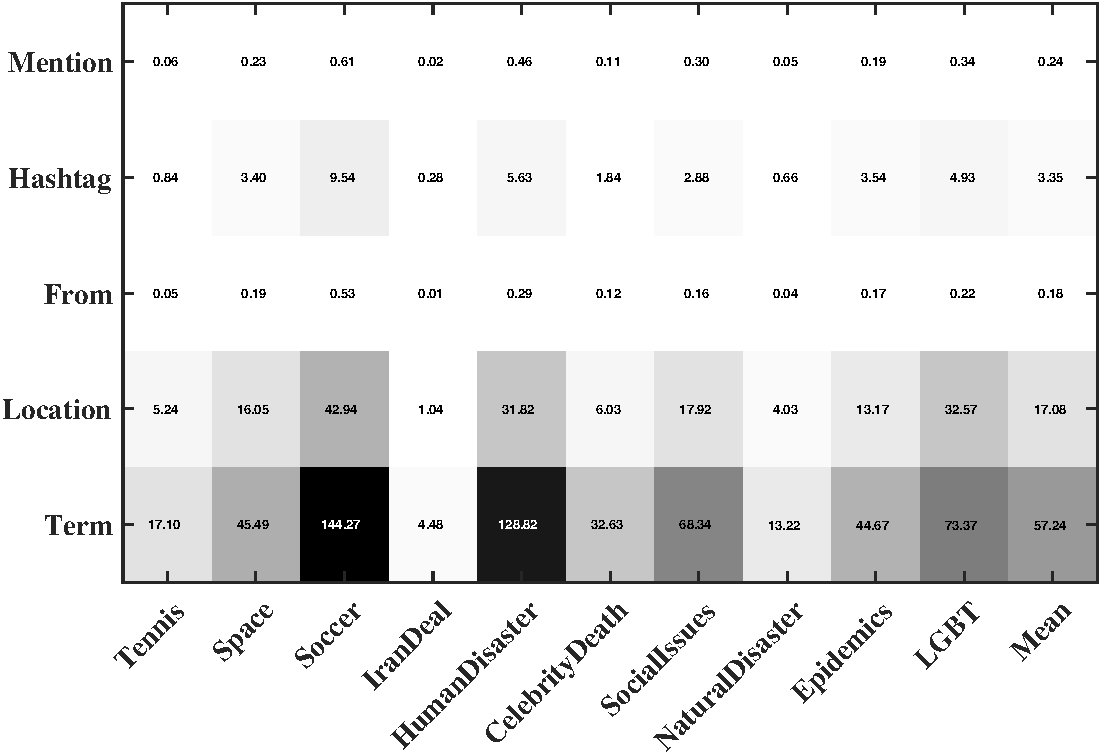
\includegraphics[width=0.5\textwidth]{images/avgMI_gray.pdf}
\vspace{-3mm}
\caption{Average MI for different features vs. Topics, last two column show mean value and stderr across all topics}
\label{fig:table1}
\end{figure}
%%%%%%%%%%%%%%%%%%%%%%%%%%%%%%%%%%%%%%%%%%%%%%%%%%%%%%%%%%%%%%%%%%%%%%%%%%%

It is important to note that due to very large amount of Term features, they were cleaned based on their frequency (having at least frequency value of 100).

\textbf{For each feature type, do any attributes correlate with importance?} In order to give a better sense of what features are better for each topic, we provided top-5 features for each topic in table \ref{table:top10MItopicsLocations}. It can be observed how different locations, hashtags, or terms showed as the top features based on mutual information are actually in relation with the specific topic.%\begin{enumerate}
%\color{red}
%\item Anecdotal feature analysis: for each of 5 feature types: (rows) top-k / median-k (?), (cols) topics -- much better than below b/c we show all topics here and we can compare features across topics.
%Don't use for now: show (rows) top-k and median-k features for different topics and (cols) 5 features (location, mention, from, term, hashtag) -- need to select a **few (2-3) interesting topics** and explain shown in table \ref{top10MItopicsLocations}
%\end{enumerate}

%%%%%%%%%%%%%%%%%%%%%%%%%%%%%%%%%%%%%%%%%%%%%%%%%%%%%%%%%%%%%%%%%%
\begin{table*}[ht]
\centering
{\renewcommand{\arraystretch}{1.2}
\resizebox{\textwidth}{!}{%
\begin{tabular}{|l|l|l|l|l|l|l|l|l|l|l|}
\hline
\textbf{Topics/Top10} & \textbf{NaturalDisaster} & \textbf{Epidemics} & \textbf{IranDeal} & \textbf{SocialIssues} & \textbf{LBGT} & \textbf{HumanCausedDisaster} & \textbf{CelebrityDeath} & \textbf{Space} & \textbf{Tennis} & \textbf{Soccer} \\ \hline
\textbf{From} & earthquake\_wo & changedecopine & mazandara & nsingerdebtpaid & eph4\_15 & ydumozyf & nmandelaquotes & daily\_astrodata & tracktennisnews & losangelessrh \\ \hline
\textbf{From} & earthalerts & drdaveanddee & hhadi119 & debtadvisoruk & mgdauber & syriatweeten & boiknox & freesolarleads & tennis\_result & shoetale \\ \hline
\textbf{From} & seelites & joinmentornetwk & 140iran & debt\_protect & stevendickinson & tintin1957 & jacanews & houston\_\_jobs & i\_roger\_federer & sport\_\_agent \\ \hline
\textbf{From} & globalfloodnews & followebola & setarehgan & negativeequityf & lileensvf1 & sirajsol & ewnreporter & star\_wars\_gifts & tennislessonnow & books\_you\_want \\ \hline
\textbf{From} & gcmcdrought & localnursejobs & akhgarshabaneh & dolphin\_ls & truckerbooman & rt3syria & paulretweet & lenautilus & kamranisbest & makeupbella \\ \hline \hline
\textbf{Hashtag} & earthquake & health & iran & ferguson & tcot & syria & rip & science & wimbledon & lfc \\ \hline
\textbf{Hashtag} & haiyan & uniteblue & irantalks & mikebrown & p2 & gaza & riprobinwilliams & starwars & usopen & worldcup \\ \hline
\textbf{Hashtag} & storm & ebola & rouhani & ericgarner & pjnet & isis & ripcorymonteith & houston & tennis & arsenal \\ \hline
\textbf{Hashtag} & tornado & healthcare & iranian & blacklivesmatter & uniteblue & israel & mandela & sun & nadal & worldcup2014 \\ \hline
\textbf{Hashtag} & prayforthephilippines & depression & no2rouhani & fergusondecision & teaparty & mh370 & nelsonmandela & sxsw & wimbledon2014 & halamadrid \\ \hline \hline
\textbf{Location} & philippines & usa & tehran & st.louis & usa & malaysia & southafrica & germany & london & liverpool \\ \hline
\textbf{Location} & ca & ncusa & u.s.a & mo & bordentown & palestine & johannesburg & roodepoort & uk & manchester \\ \hline
\textbf{Location} & india & garlandtx & nederland & usa & newjersey & syria & capetown & houston & india & london \\ \hline
\textbf{Location} & newdelhi & oh-sandiego & iran & dc & sweethomealabama! & israel & pretoria & austin & pakistan & nigeria \\ \hline
\textbf{Location} & newzealand & washington & globalcitizen & washington & aurora & london & durban & tx & islamabad & india \\ \hline \hline
\textbf{Mention} & oxfamgb & foxtramedia & 4freedominiran & deray & jjauthor & ifalasteen & nelsonmandela & bizarro\_chile & wimbledon & lfc \\ \hline
\textbf{Mention} & weatherchannel & obi\_obadike & iran\_policy & natedrug & 2anow & revolutionsyria & realpaulwalker & nasa & usopen & arsenal \\ \hline
\textbf{Mention} & redcross & who & hassanrouhani & antoniofrench & govchristie & drbasselabuward & robinwilliams & j\_ksen & andy\_murray & realmadriden \\ \hline
\textbf{Mention} & twcbreaking & obadike1 & un & bipartisanism & a5h0ka & mogaza & rememberrobin & jaredleto & serenawilliams & ussoccer \\ \hline
\textbf{Mention} & abc7 & c25kfree & statedept & theanonmessage & barackobama & palestinianism & tweetlikegiris & 30secondstomars & espntennis & mcfc \\ \hline \hline
\textbf{Term} & philippines & health & iran & police & obama & israel & robin & cnblue & murray & madrid \\ \hline
\textbf{Term} & donate & ebola & regime & protesters & gun & gaza & williams & movistar & tennis & goal \\ \hline
\textbf{Term} & typhoon & acrx & nuclear & officer & rights & israeli & nelson & enero & federer & cup \\ \hline
\textbf{Term} & affected & medical & iranian & protest & america & killed & mandela & ΍imperdible & djokovic & manchester \\ \hline
\textbf{Term} & relief & virus & resistance & cops & gop & children & cory & greet & nadal & match \\ \hline
\end{tabular}
}}
\caption{Top 5 features for each topic based on Mutual Information}
\label{table:top10MItopicsLocations}
\end{table*}
%%%%%%%%%%%%%%%%%%%%%%%%%%%%%%%%%%%%%%%%%%%%%%%%%%%%%%%%%%%%%%%%%%

\textcolor{red}{
\textbf{\color{red}scatterplots of feature MI -- the absolute last thing we do (density plots?!!)}
**which plots below, and for which topics?  Could pick out most useful features for topics in part (a)(i) and just show selected scatter plots below for these feature types.
from, mention MIs vs. {followers, favorites, friends, hashtags, tweets}
hashtag MI vs. {\#tweets, \#users}
location MI vs. {\#users}
term MI vs. {\#tweets}
}

%%%%%%%%%%%%%%%%%%%%%%%%%%%%%%%%%%%%%%%%%%%%%%%%%%%%%%%%%%%%%%%%%%%%%%%%%%%
\begin{figure*}[tbph!]
\centering
\begin{tabular}{ccccc}
\begin{tabular}{ccccc}
\subfloat[Fig:][Favorite Count]{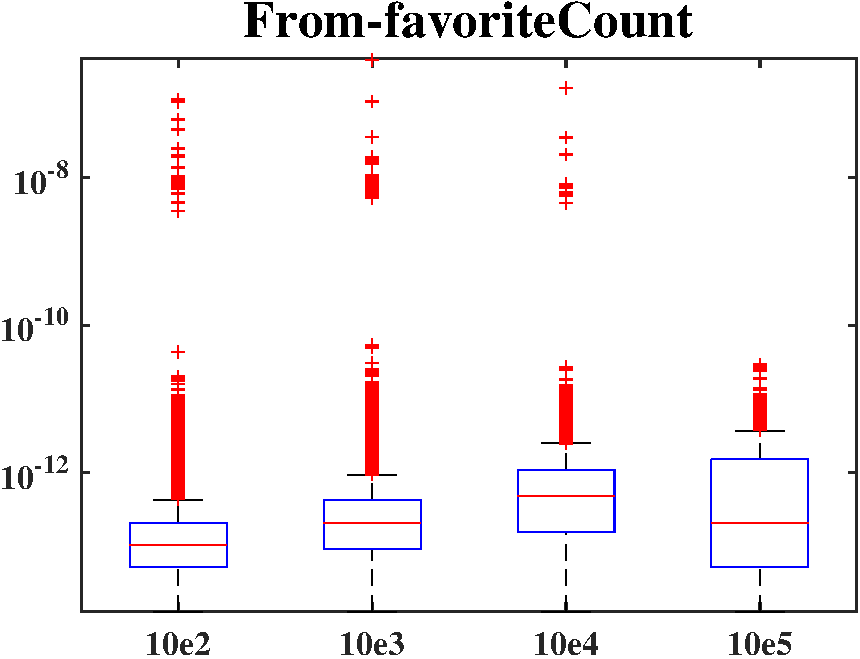
\includegraphics[width=32mm, height=35mm]{images/BoxPlots_IranDeal/From-favoriteCount.pdf}}
\subfloat[Fig:][Followers Count]{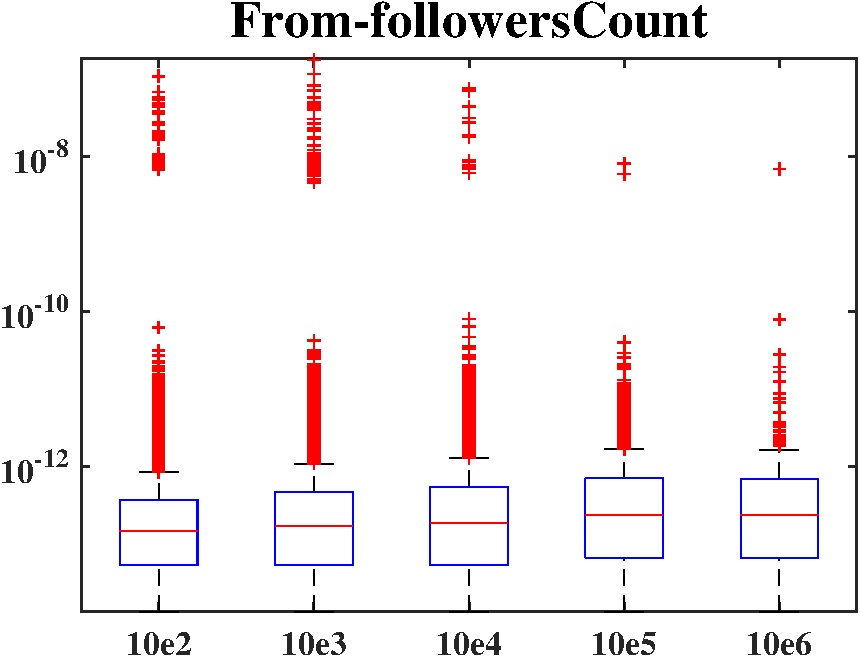
\includegraphics[width=32mm, height=35mm]{images/BoxPlots_IranDeal/From-followersCount.pdf}}
\subfloat[Fig:][Friends Count]{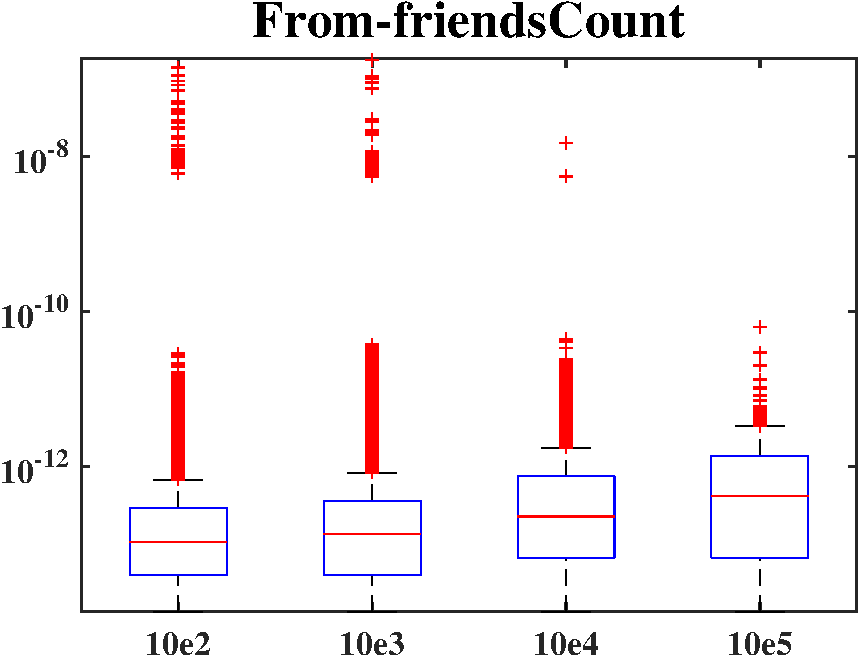
\includegraphics[width=32mm, height=35mm]{images/BoxPlots_IranDeal/From-friendsCount.pdf}}
\subfloat[Fig:][Hashtag Count]{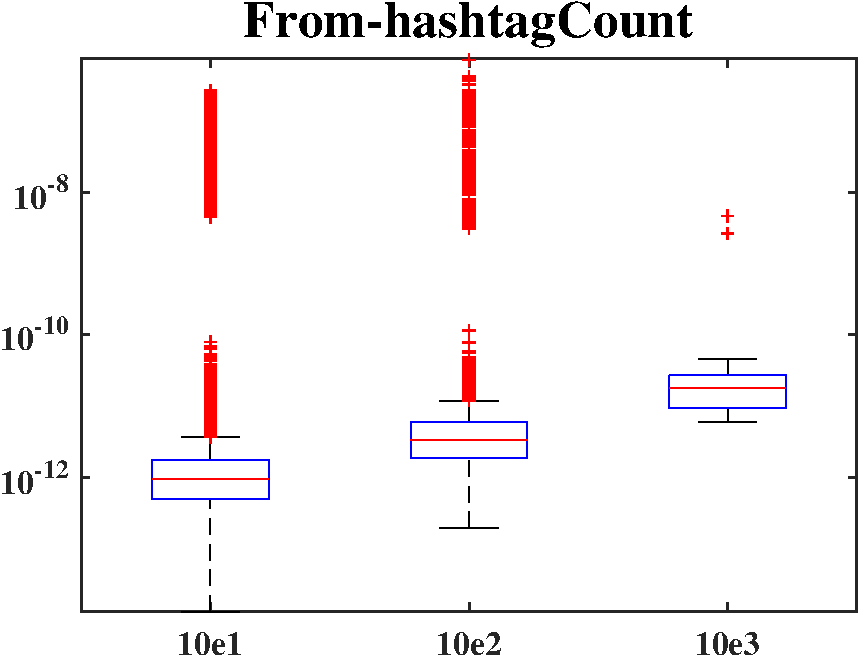
\includegraphics[width=32mm, height=35mm]{images/BoxPlots_IranDeal/From-hashtagCount.pdf}}
\subfloat[Fig:][Tweet Count]{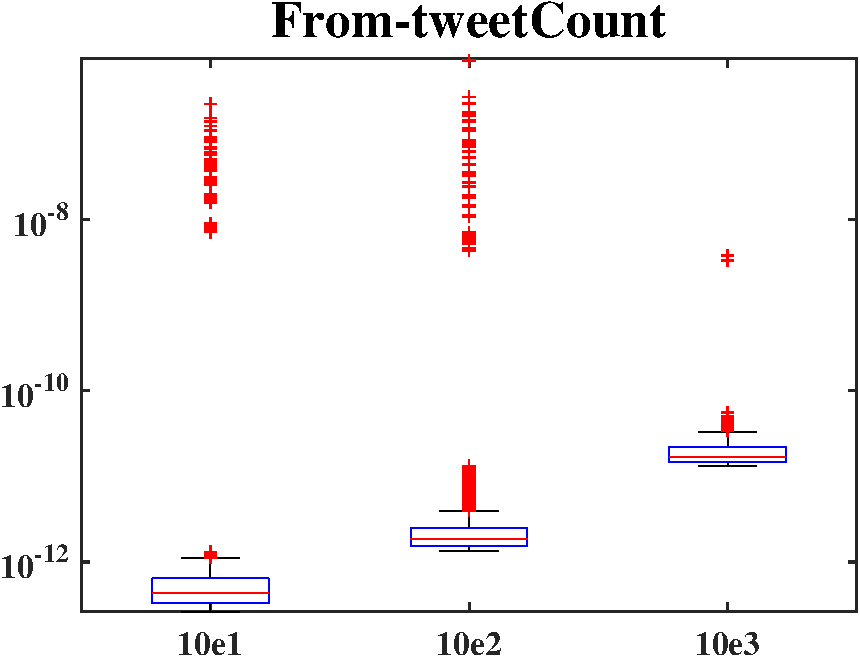
\includegraphics[width=32mm, height=35mm]{images/BoxPlots_IranDeal/From-tweetCount.pdf}} \\
%\vspace{-10mm}
\subfloat[Fig:][Tweet Count]{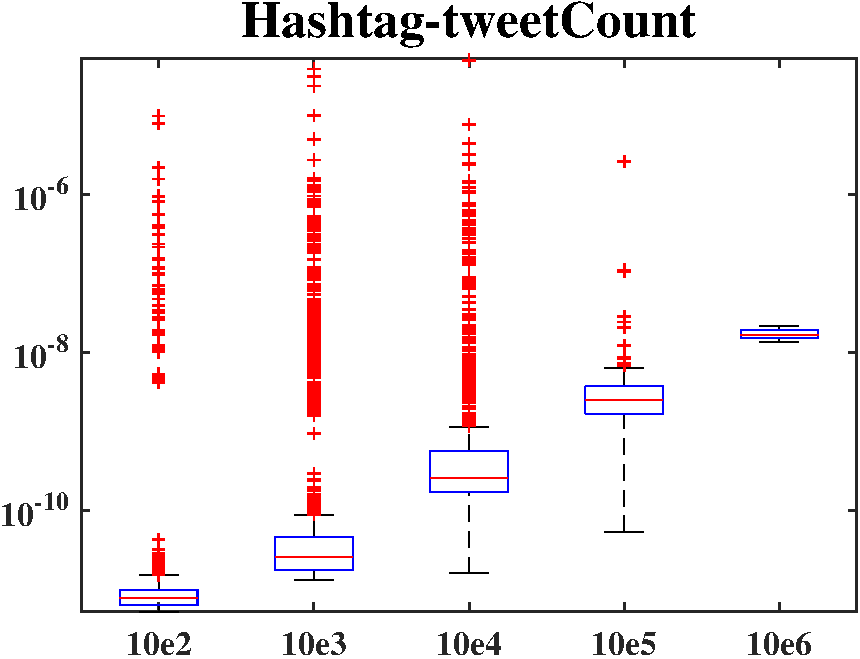
\includegraphics[width=32mm, height=35mm]{images/BoxPlots_IranDeal/Hashtag-tweetCount.pdf}}
\subfloat[Fig:][User Count]{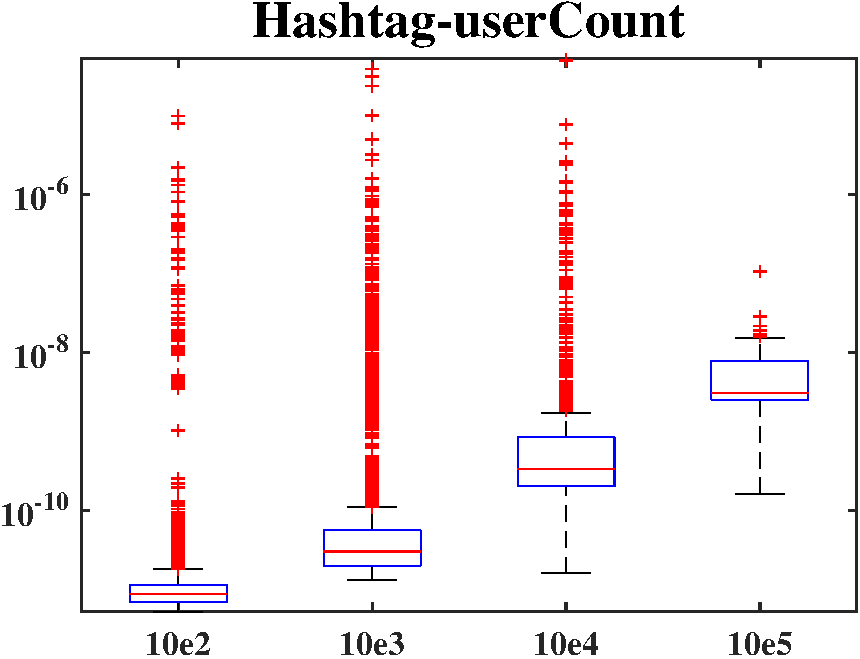
\includegraphics[width=32mm, height=35mm]{images/BoxPlots_IranDeal/Hashtag-userCount.pdf}}
\subfloat[Fig:][User Count]{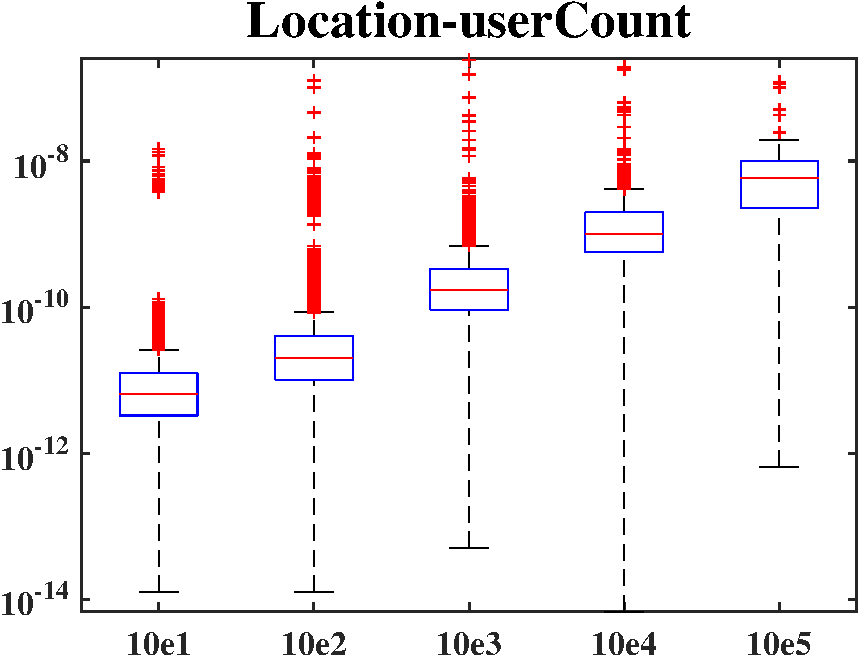
\includegraphics[width=32mm, height=35mm]{images/BoxPlots_IranDeal/Location-userCount.pdf}}
\subfloat[Fig:][Tweet Count]{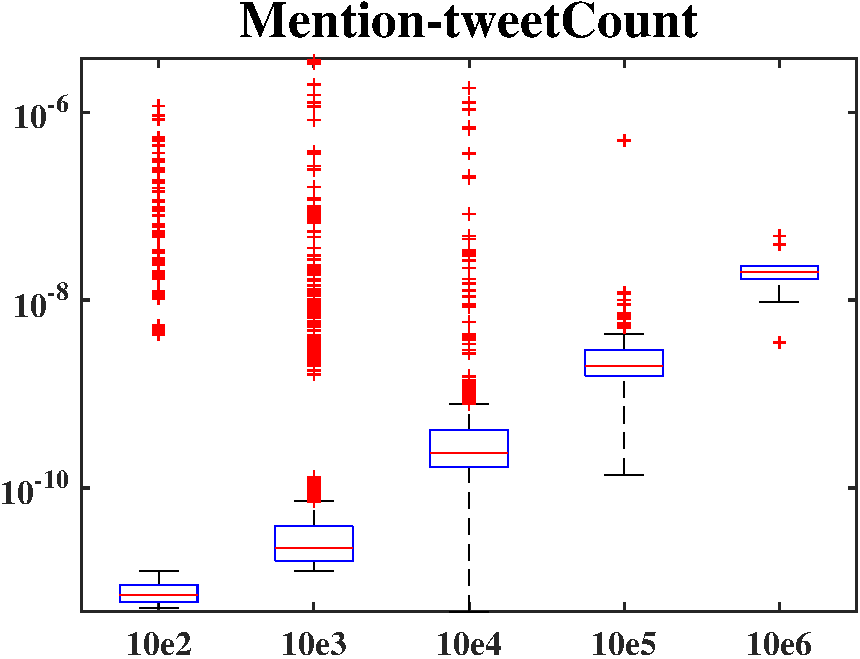
\includegraphics[width=32mm, height=35mm]{images/BoxPlots_IranDeal/Mention-tweetCount.pdf}}
\subfloat[Fig:][Tweet Count]{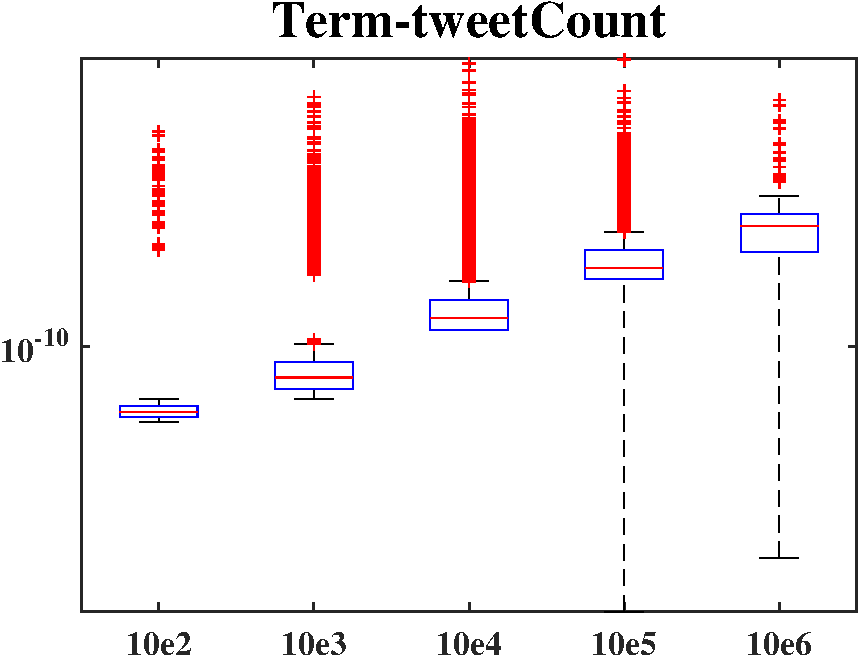
\includegraphics[width=32mm, height=35mm]{images/BoxPlots_IranDeal/Term-tweetCount.pdf}} \\
\end{tabular}
\end{tabular}
\vspace{-2mm}
\caption {Box Plots for feature attributes counts vs. MI. Top row shows attributes \{favoriteCount, followerCount, friendCount, hashtagCount, tweetCount\} for $From$ feature. Bottom row shows attributes tweetCount and/or userCount for $Hashtag$, $Location$, $Mention$,and $Term$ features.}
\label{fig:boxplots2}
\end{figure*}
%%%%%%%%%%%%%%%%%%%%%%%%%%%%%%%%%%%%%%%%%%%%%%%%%%%%%%%%%%%%%%%%%%%%%%%%%%%


%%%%%%%%%%%%%%%%%%%%%%%%%%%%%%%%%%%%%%%%%%%%%%%%%%%%%%%%%%%%%%%%%%%%%%%%%%%
\begin{figure*}[tbph!]
\centering
\begin{tabular}{ccccc}
\begin{tabular}{ccccc}
\subfloat[Fig:][Favorite Count]{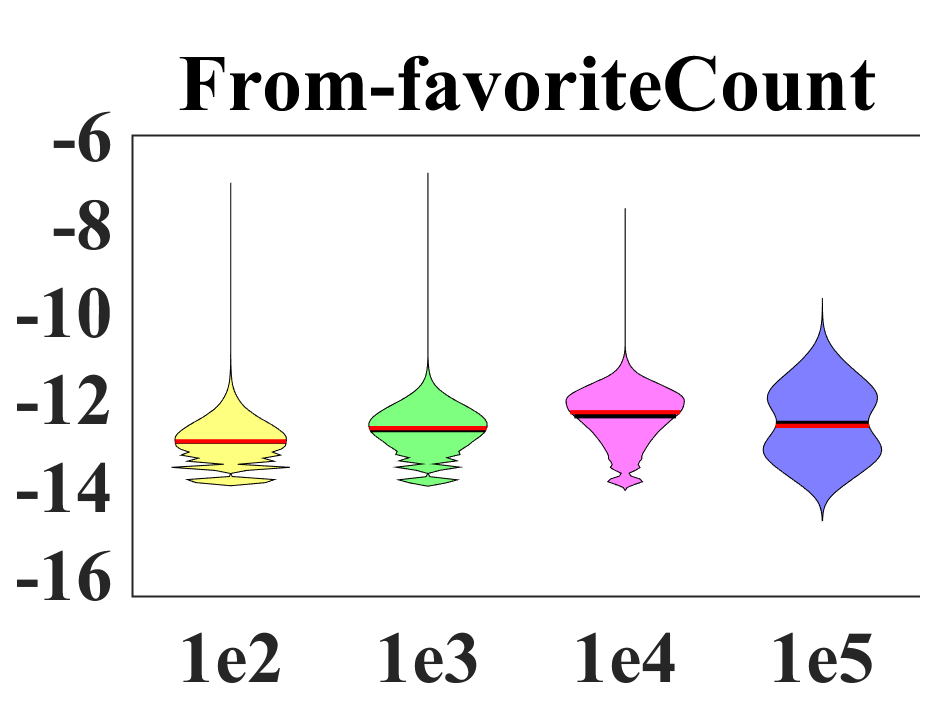
\includegraphics[width=32mm, height=35mm]{images/ViolinPlots/From-favoriteCount.eps}}
\subfloat[Fig:][Followers Count]{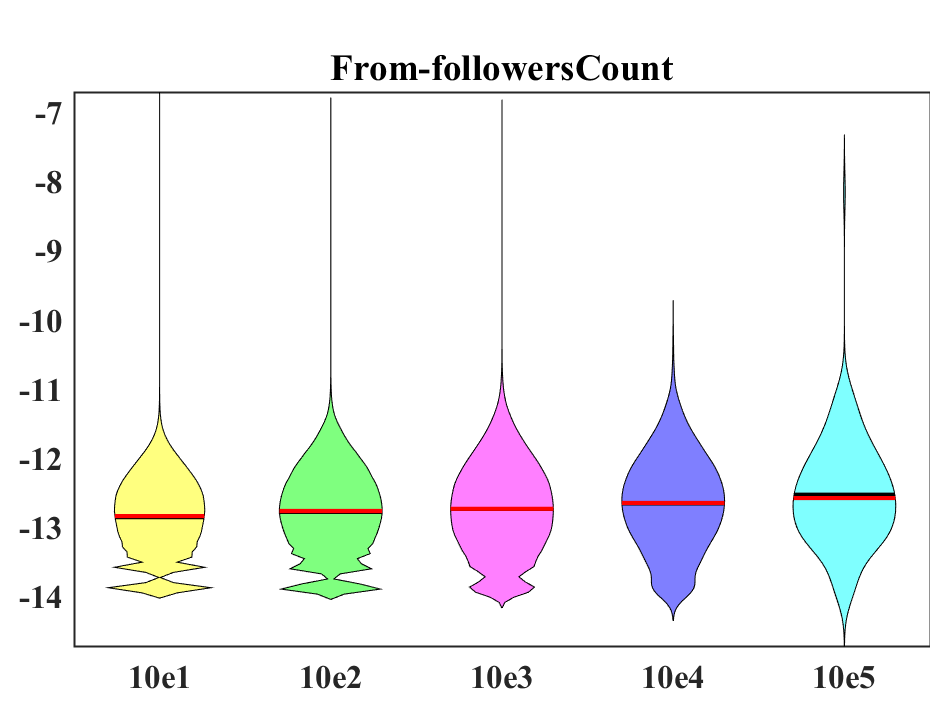
\includegraphics[width=32mm, height=35mm]{images/ViolinPlots/From-followersCount.eps}}
\subfloat[Fig:][Friends Count]{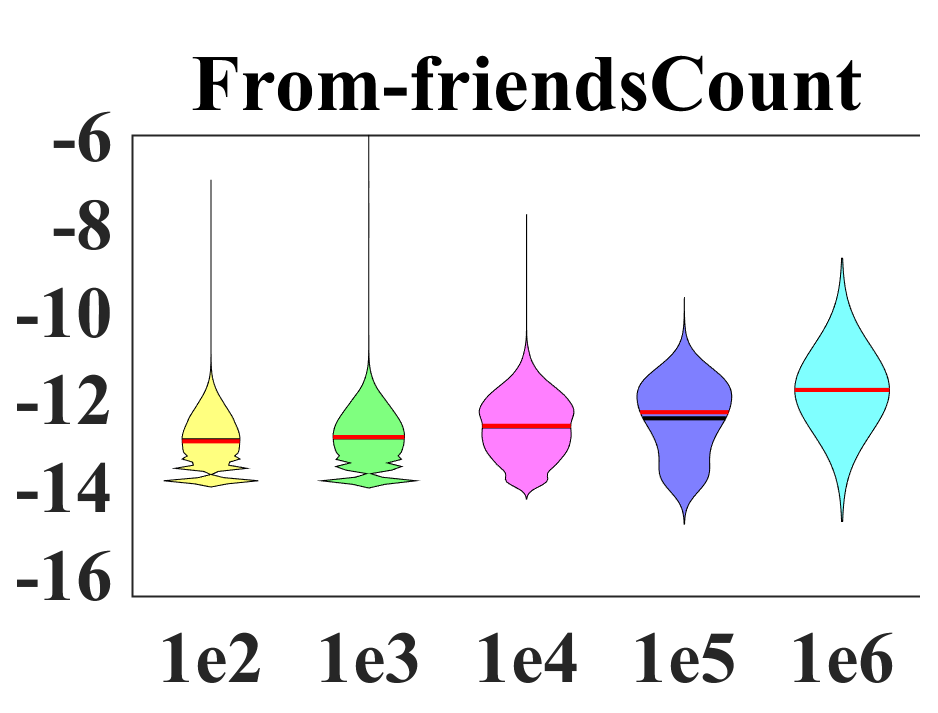
\includegraphics[width=32mm, height=35mm]{images/ViolinPlots/From-friendsCount.eps}}
\subfloat[Fig:][Hashtag Count]{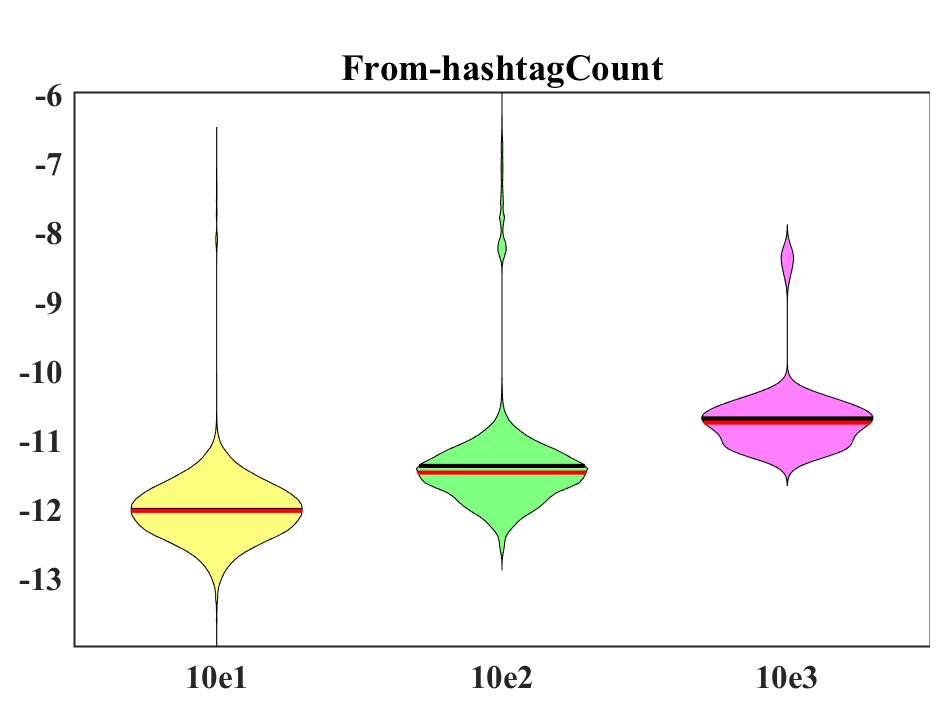
\includegraphics[width=32mm, height=35mm]{images/ViolinPlots/From-hashtagCount.eps}}
\subfloat[Fig:][Tweet Count]{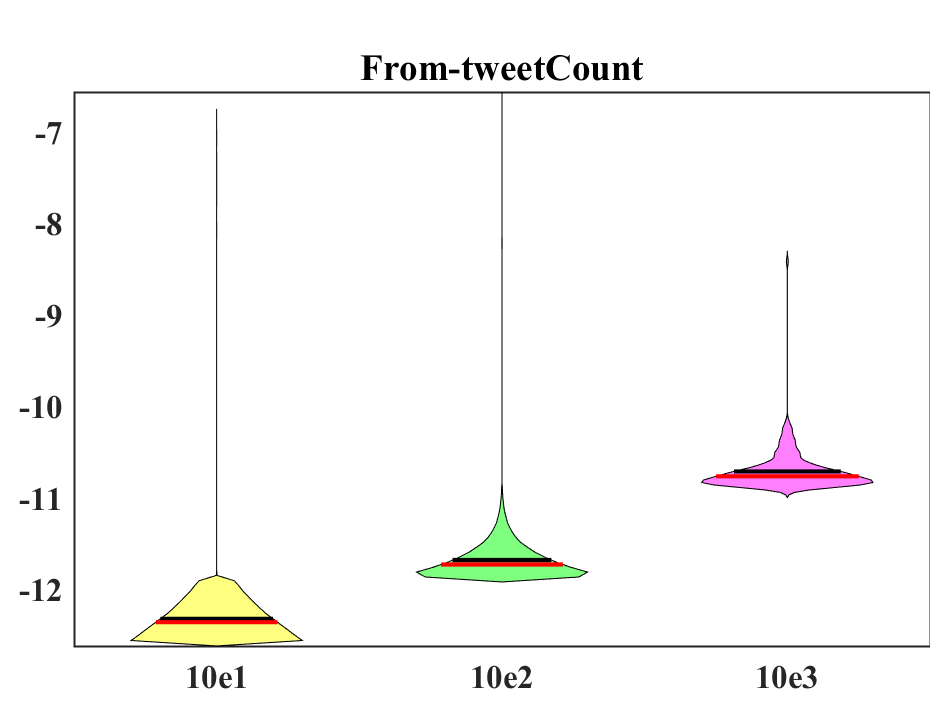
\includegraphics[width=32mm, height=35mm]{images/ViolinPlots/From-tweetCount.eps}} \\
%\vspace{-10mm}
\subfloat[Fig:][Tweet Count]{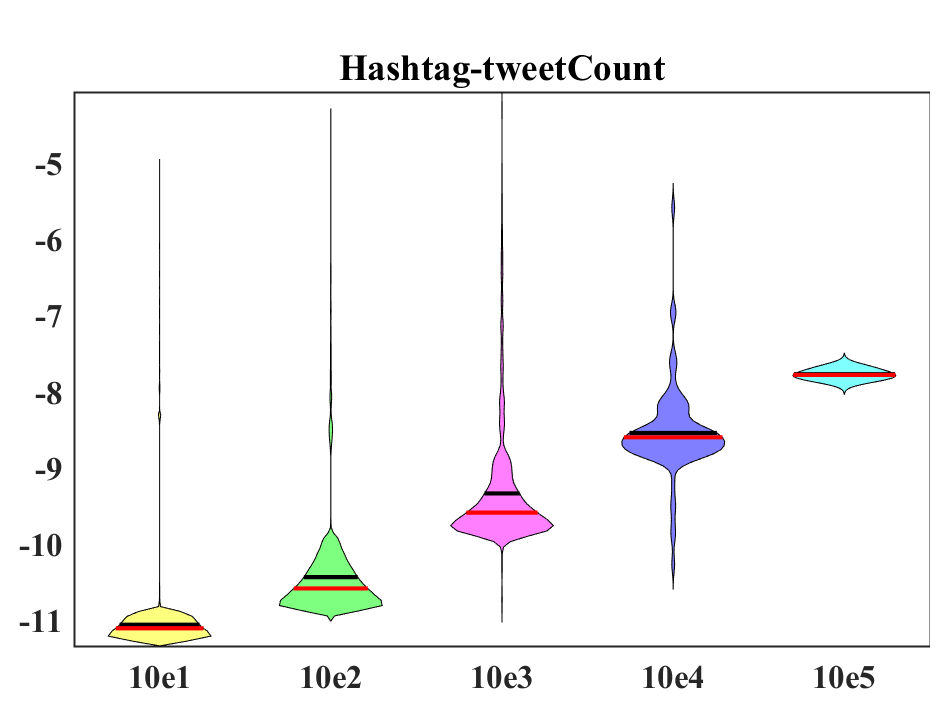
\includegraphics[width=32mm, height=35mm]{images/ViolinPlots/Hashtag-tweetCount.eps}}
\subfloat[Fig:][User Count]{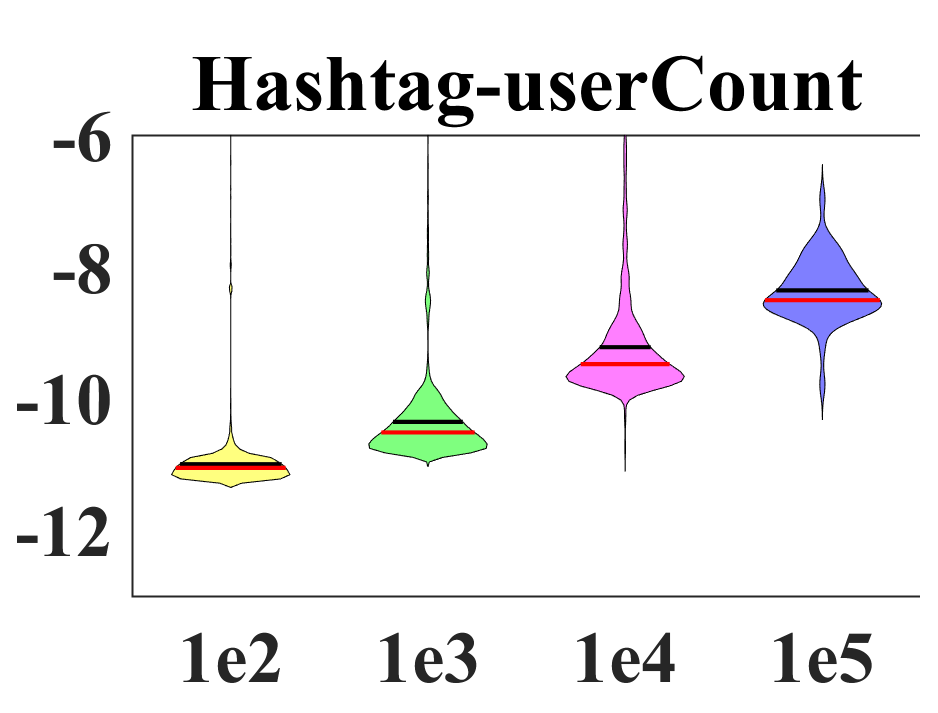
\includegraphics[width=32mm, height=35mm]{images/ViolinPlots/Hashtag-userCount.eps}}
\subfloat[Fig:][User Count]{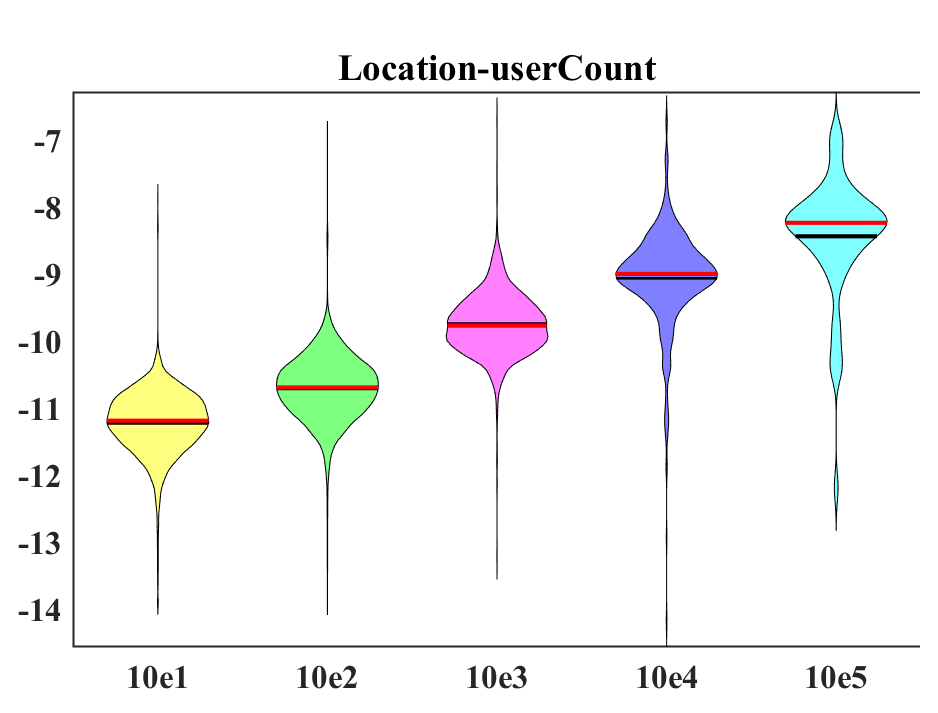
\includegraphics[width=32mm, height=35mm]{images/ViolinPlots/Location-userCount.eps}}
\subfloat[Fig:][Tweet Count]{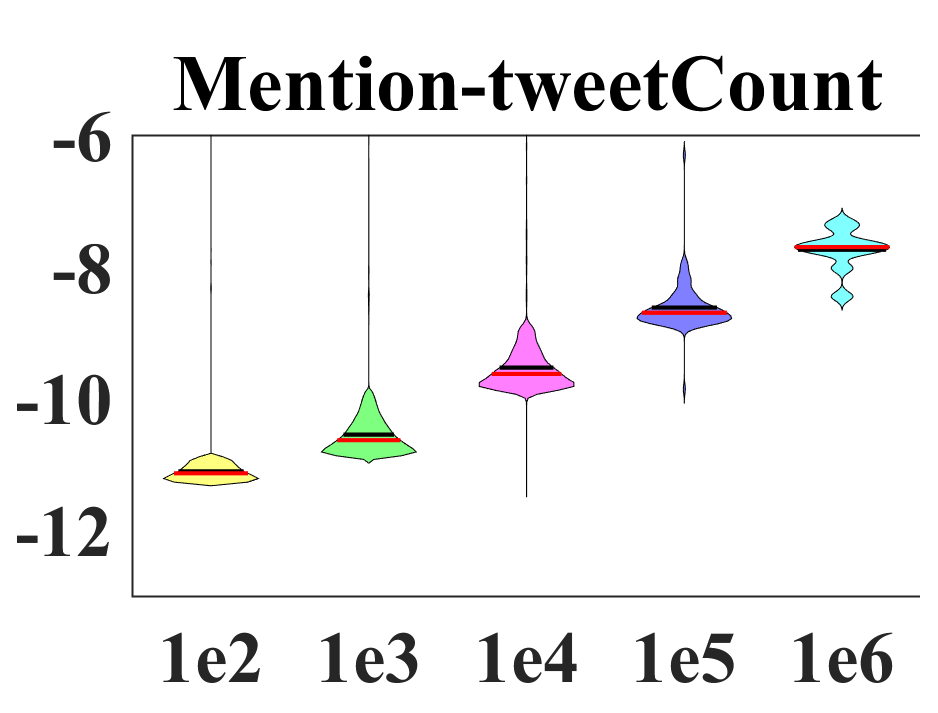
\includegraphics[width=32mm, height=35mm]{images/ViolinPlots/Mention-tweetCount.eps}}
\subfloat[Fig:][Tweet Count]{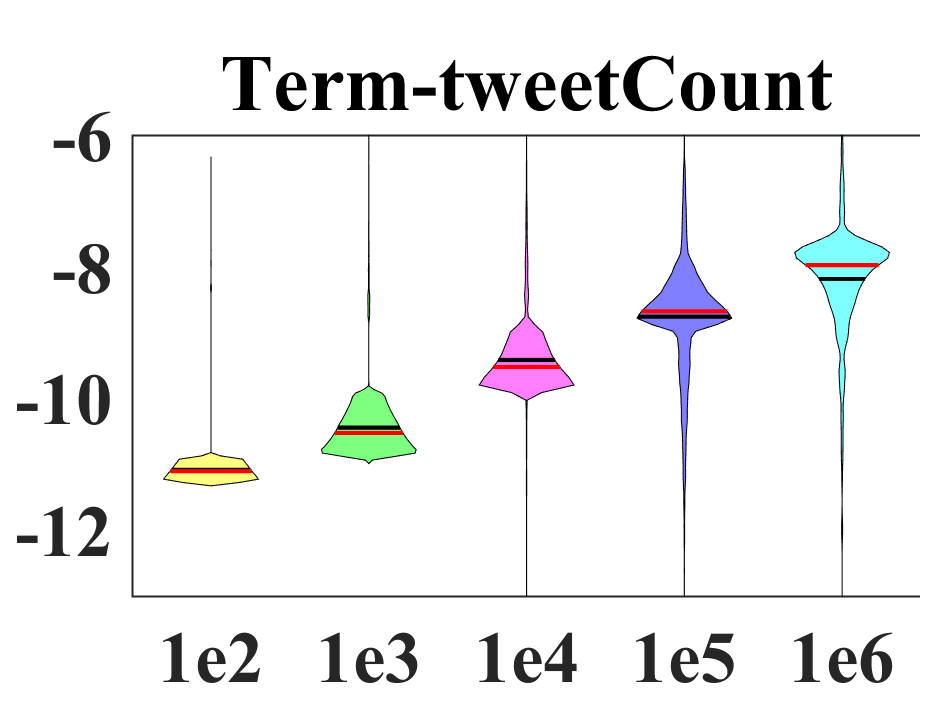
\includegraphics[width=32mm, height=35mm]{images/ViolinPlots/Term-tweetCount.eps}} \\
\end{tabular}
\end{tabular}
\vspace{-2mm}
\caption {ViolinPlots for feature attributes counts vs. MI. Top row shows attributes \{favoriteCount, followerCount, friendCount, hashtagCount, tweetCount\} for $From$ feature. Bottom row shows attributes tweetCount and/or userCount for $Hashtag$, $Location$, $Mention$,and $Term$ features.}
\label{fig:violinplots}
\end{figure*}
%%%%%%%%%%%%%%%%%%%%%%%%%%%%%%%%%%%%%%%%%%%%%%%%%%%%%%%%%%%%%%%%%%%%%%%%%%%


%%%%%%%%%%%%%%%%%%%%%%%%%%%%%%%%%%%%%%%%%%%%%%%%%%%%%%%%%%%%%%%%%%%%%%%%%%%
\begin{figure*}[tbph!]
\centering
\begin{tabular}{cccc}
\subfloat[Fig:][]{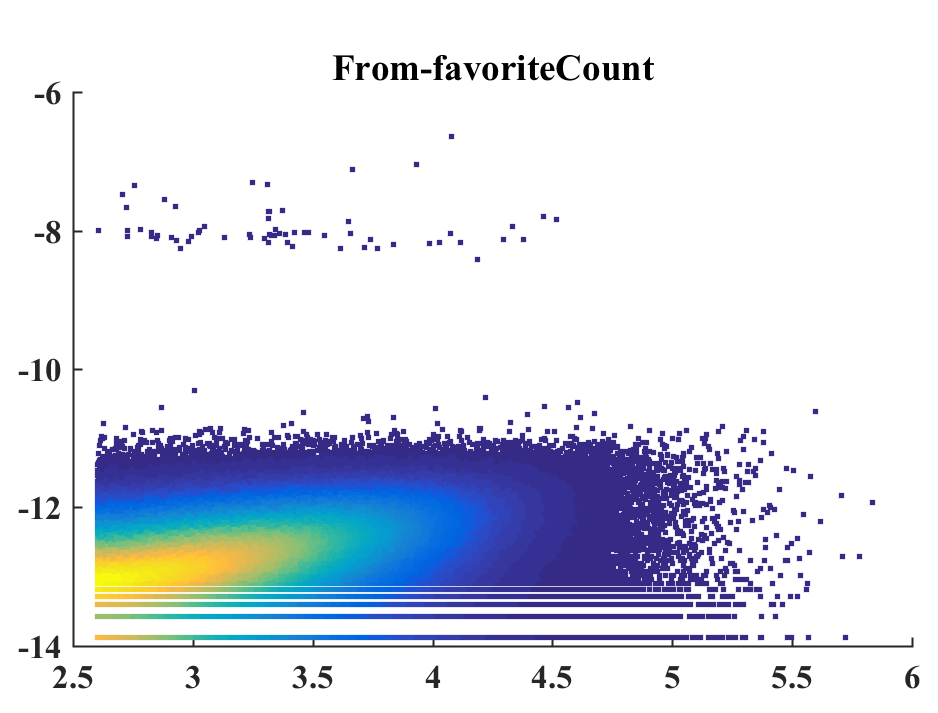
\includegraphics[width=40mm, height=35mm]{images/DensityPlots_IranDeal/dscatterPlot_From_favoriteCount.eps}}
\subfloat[Fig:][]{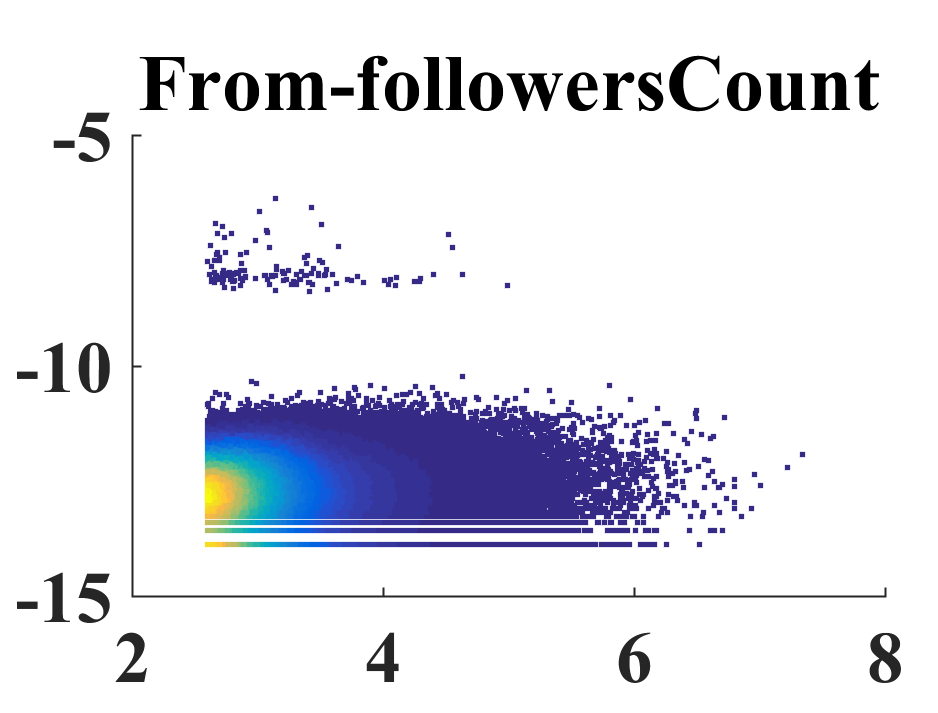
\includegraphics[width=40mm, height=35mm]{images/DensityPlots_IranDeal/dscatterPlot_From-followersCount.eps}}
\subfloat[Fig:][]{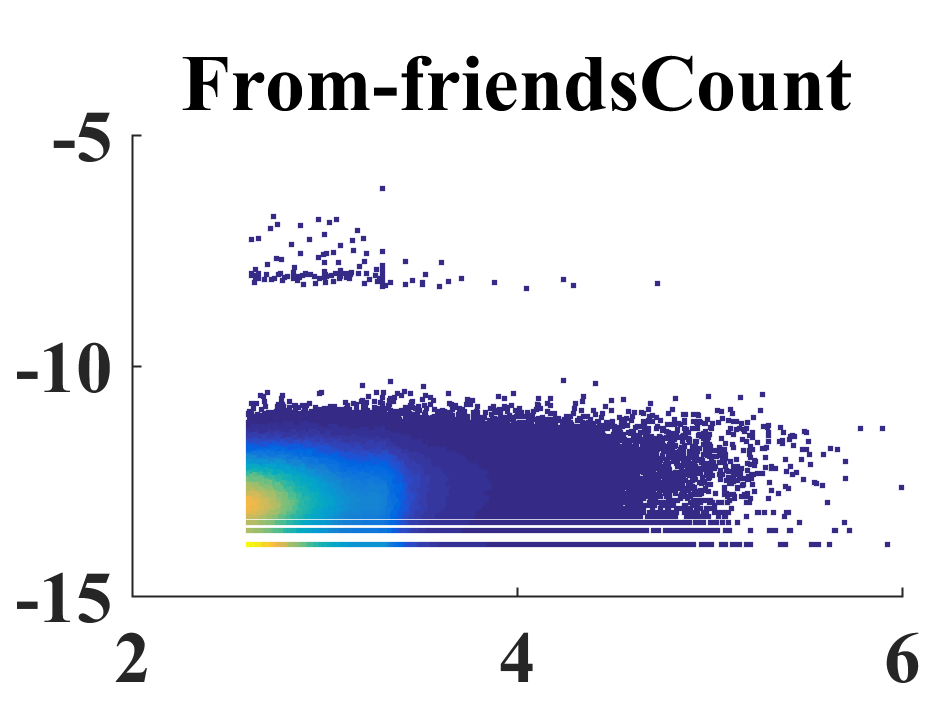
\includegraphics[width=40mm, height=35mm]{images/DensityPlots_IranDeal/dscatterPlot_From-friendsCount.eps}}
\subfloat[Fig:][]{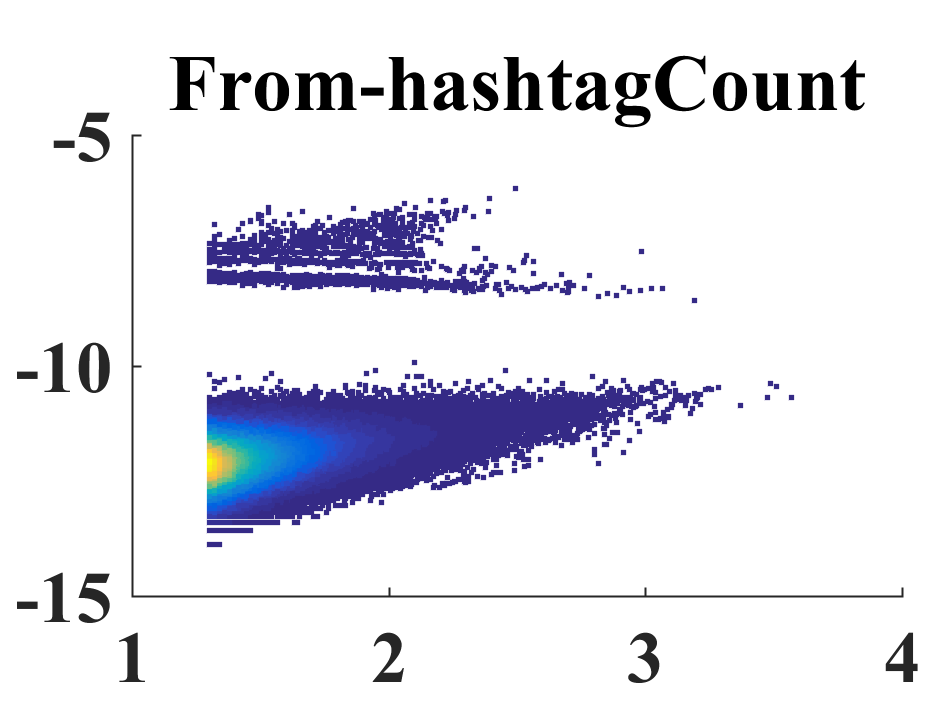
\includegraphics[width=40mm, height=35mm]{images/DensityPlots_IranDeal/dscatterPlot_From-hashtagCount.eps}} \\
\end{tabular}
\vspace{-2mm}
\caption {DensityPlots for feature attributes counts vs. MI. (a-d) show attributes \{favoriteCount, followerCount, friendCount, hashtagCount\} for $From$ feature}
\label{Fig3}
\end{figure*}
%%%%%%%%%%%%%%%%%%%%%%%%%%%%%%%%%%%%%%%%%%%%%%%%%%%%%%%%%%%%%%%%%%

\section{Related Works}
%%%%%%%%%%%%%%% TWITTER CURRENT SEARCH METHOD %%%%%%%%%%%%%%%%%
\iffalse
Twitter Search : https://blog.twitter.com/2011/the-engineering-behind-twitter-s-new-search-experience

Twitter model: reverse indexes was built in MySQL, leveraging its concurrent transactions and B-tree data structures to support indexing and searching partitioned across multiple databases. Earlybird, a real-time reverse index based on Lucene, gave much better performance and memory efficiency than MySQL for real-time search. 
"There is a lot of information on Twitter — on average, more than 2,200 new Tweets every second! During large events, for example the \#tsunami in Japan, this rate can increase by 3 to 4x. Often, users are interested in only the most memorable Tweets or those that other users engage with. In our new search experience, we show search results that are most relevant to a particular user. So search results are personalized, and we filter out the Tweets that do not resonate with other users."

Supporting personalized search, they needed three types of signal: Static signals at indexing time, Resonance signals updated over time, Information about the searcher at search time. At indexing time, tweets are annotated with static information about the user and the language of the tweet's text. Dynamic updates, such as users' interactions with tweets are made over time. At query time, user's social graph is passed along the user's query. A specialized ranking function is used to combine relevance signals and the social graph for computing personalized relevance score for each tweet. The results consists of highest-ranking, most-recent tweets. The ranking function accesses the social graph and uses knowledge about the relationship between the searcher and the author of a tweet during ranking.
\fi
%%%%%%%%%%%%%%%%%%%%%%%%%%%%%%%%%%%%%%%%%%%%%%%%%%%%%%

This section provides existing research on the use of social media as a sensor for topic detection on social media. Here, we focus on related research on both events and topics detection from social media since events are special type of topics and can be considered as a topic.

Historically, event detection has been studied extensively in text mining, NLP, and IR to find events from conventional media sources such as news streams \cite{yang}. With the growth of social media sites such as Facebook, Twitter and other microblogs, social media sites have become known as powerful communication tools for sharing and exchanging information about such events. To see how different works address topic detection on social media, we focus on the two highly studied types of topic detections: Trending Topic Detection, Event Detection.
%%%%% TRENDING TOPIC DETECTION
First group of works focus on trending topic detection methods. Majority of works on detecting trending topics use bursts as the indicator of events, where a burst is defined as a sudden change in posting rates of some keywords, hashtags, etc. These can further be divided into multiple categories based on how they use bursts to extract the event. First category, clustering-based methods, focus on the hypothesis that trends are topical and topics are defined by collection of relevant content, hence trends can be detected by clustering content. \cite{wei} proposed a graphical model to discover latent events clustered in the spatial, temporal and lexical dimensions. \cite{yamamoto} focus on the task of multi-label classification of tweets into living aspects such as eating.%They use hierarchical estimation framework to estimate aspects of unknown tweets. This task is formulated into two phase of extracting topics from set of tweets using LDA and  calculating relevance between topics and aspects of tweets with computing Shannon entropy of each association.
 \cite{petrovic,ishikawa,murata,becker,tweetmotif,wangLee}. Second category, term-based methods focus on the hypothesis that topics can be detected by focusing on temporal patterns of terms/keywords independent of contents of documents \cite{mathioudakis,cuiZhang,zhaoSports,nichols}. Third category, query-based methods, focus on the hypothesis that trending topics can be detected by measuring user-defined criteria \cite{albakour,sakakiDrive}. Last work, network Structure-based method, focused on the hypothesis that trending topics can be detected by studying the network structure of users \cite{budak}.

However, trending topics detection methods are not targeted. Our method differs from trending topic detection methods in the sense that we are focusing on a set of topics that can not necessarily be detected using burst.

%%%%% TARGETED SPECIFIC TOPIC DETECTION
Second groups of works focus on detection of a specific targeted topic such as disaster or epidemic. Regarding disaster, predictive studies \cite{sandy}, studied the network of users and focused on choosing the best groups of users in order to achieve lead-times i.e. faster detection of disastrous event (following the concept of "friendship paradox"\footnote{On average, most people have fewer friends than their friends have}). \cite{sakakiEq2} used SVM classifier for detecting earthquakes and employed location estimation method such as Kalman Filtering for localizing it. \citeauthor{sakakiEq2} extracted statistical features e.g., the number and position of words in a tweet, keyword features and word context features. These studies investigated the real-time nature of Twitter and provided promising results. However another set of works focused on descriptive studies on disaster by discussing the behavior of Twitter users during crisis \cite{vieweg,cheong,starbird} and do not address exploiting detection of crisis events. They investigated the use of social media during crisis in order to identify information propagation properties, social behavior of users e.g. retweeting behavior, information contributing to situational awareness, and active players in communicating information. However, this behavioral information could be exploited in development of sensors.

Regarding health epidemic detection, researchers used content-based method and/or structure-based methods. Content-based methods, \cite{culotta} and \cite{aramaki} both tried to identify influenza-related tweets and find correlations of these tweets to CDC statistics.  Both works extracted bag-of-words as features. As for methodology, the former used single and multiple linear regression showing that multiple linear regression works better, while the latter employed SVM. Results showed high correlation of their estimation of influenza in early stages with values from U.S CDC and Japan's Infection Disease Surveillance Center. Structure-based method, \cite{garcia} use the friendship paradox concept \cite{feld} for early detection of contagious outbreaks. They provided a method for choosing sensor groups from friends of random sets of users to find more central individuals in order to enforce early detection. They claim that this sensor group represents more central individuals and individuals at the center of a network are likely to receive a contagion sooner than randomly-chosen members of the population (because central individuals are a smaller number of steps away from the average individual in the network). As a result, \cite{garcia} argued that this selection process of sensor groups helps in early detection of outbreaks.

On the other hand, hybrid methods \cite{sadilek} ,exploited both content of tweets and structural information of users network. They employed a semi-supervised approach to learn a SVM classifier using n-grams as features in order to detect ill individuals. Then, they estimated physical interaction between healthy and sick people based on co-location and friendship. This enabled them to study the effect of these two factors of social activity (co-location for contact network and friendship for social ties) on public health.

These method focus on finding a specific topic, thus using a very primitive method for curating the data e.g., querying keyword "earthquake". In addition, there is no discussion on how can these methods be generalized for other topics.

%%%%% TWEET RECOMMENDATION
In a more similar settings, \cite{Krestel} compared four different methods of language model, topic model, logistic regression and boosting to evaluate recommended tweets for a given news article on a dataset of 55k news articles and 121k tweets. \cite{Yan,chen} focus on tweet recommendation based on user preferences and tweet popularity, thus focusing on user's own tweet history, retweet history and social relations between users as features. 




\section{Conclusions}

\section{Acknowledgments}

\section{Copyright}

\bibliographystyle{aaai}
\bibliography{mybib.bib}

\end{document}
